\documentclass[11pt]{article}

\usepackage[a4paper,margin=1in]{geometry}
\usepackage[T1]{fontenc}
\usepackage[utf8]{inputenc}
\usepackage{lmodern}
\usepackage{microtype}
\usepackage{amsmath}
\usepackage{amssymb}
\usepackage{booktabs}
\usepackage{graphicx}
\usepackage{multirow}
\usepackage{siunitx}
\usepackage{hyperref}
\usepackage{enumitem}

\hypersetup{
    colorlinks=true,
    linkcolor=blue,
    urlcolor=blue
}

\sisetup{
    detect-all,
    group-separator={,},
    group-minimum-digits=4,
    scientific-notation=false
}

\title{Evaluating Variable Timing in Spiking Neural Networks\\Under Clean and Adversarial Training}
\author{Working Draft}
\date{\today}

\begin{document}
\maketitle

\begin{abstract}
Variable Timing (VT) allows a spiking neural network (SNN) to stop inference early once it becomes sufficiently confident, potentially reducing computation without retraining the backbone. This paper does not propose a new VT mechanism. Instead, it asks a narrower question: when VT is compared fairly against fixed-time truncation at similar clean compute budgets, what does it actually buy, and does any such advantage extend from clean efficiency to adversarial robustness? We study two deterministic SNN backbones with direct input encoding and standard leaky integrate-and-fire dynamics: a vanilla ResNet-18-style model and a vanilla VGG16-style model. VT is compared against compute-matched fixed-time baselines using SynOps as the primary compute metric. On both backbones, VT substantially improves the clean accuracy--compute frontier relative to matched fixed-time truncation. For example, on the clean-trained VGG16 checkpoint, the calibration-selected VT policy reaches \SI{86.99}{\percent} test accuracy at \num{65.2}\,M SynOps, compared with \SI{80.50}{\percent} for the compute-matched fixed-$T=3$ baseline and \SI{88.20}{\percent} for full $T=8$ inference. On the adversarially trained ResNet-18 checkpoint, the selected VT policy reaches \SI{71.48}{\percent} at \num{163.3}\,M SynOps, compared with \SI{69.35}{\percent} for the matched fixed-$T=4$ baseline and \SI{73.67}{\percent} for full $T=8$ inference. Robustness, however, is not improved in any simple way. Clean-trained checkpoints collapse under strong attacks regardless of the inference policy. Adversarially trained checkpoints show a mixed picture: VT can look competitive under PGD, but under AutoAttack matched fixed-time baselines remain stronger. The resulting conclusion is that VT is a strong clean adaptive-inference tool, but its added value is clearest on the clean efficiency frontier rather than on adversarial robustness.
\end{abstract}

\section{Introduction}
Spiking neural networks process information over discrete simulation steps rather than in a single feed-forward pass. That temporal structure makes adaptive inference unusually natural: if a sample becomes easy early, should the network continue consuming its full time budget? Variable Timing (VT) addresses this by stopping inference once confidence crosses a threshold. If effective, VT offers a straightforward way to reduce latency and spike-driven computation without redesigning the backbone.

The problem is that VT is easy to oversell. A VT policy can look impressive when compared only against full-horizon inference, even if a short fixed-time model would already give a similar trade-off. Likewise, robustness claims can be misleading when they are evaluated under only one training regime or one attack. The precise gap, therefore, is not the existence of VT as an idea, but the lack of controlled evidence about what VT actually adds beyond static truncation once the comparison is made fairly.

That gap matters because VT is fundamentally a systems mechanism rather than a stand-alone classifier. Its value depends on whether it produces a better accuracy--compute trade-off than simple truncation, and whether any favorable behavior survives under strong robustness evaluation. If those questions are left ambiguous, it becomes hard to know whether VT is genuinely exploiting per-sample difficulty or merely benefiting from a favorable but unfair comparison.

This paper studies that question directly. We do not propose a new VT mechanism. Instead, we evaluate a confidence-based VT policy on two deterministic backbones, vanilla ResNet-18 and vanilla VGG16, under two regimes: clean training and full adversarial training. Thresholds are selected on calibration, VT is compared against compute-matched fixed-$T$ baselines using SynOps, and robustness is tested with both PGD and AutoAttack.

The answer is mixed but coherent. VT clearly improves the clean accuracy--compute frontier in both regimes, and it does so relative to the fair baseline that matters most: compute-matched fixed-time truncation. On the clean-trained model, the selected VT policy retains most of the full-horizon clean accuracy while strongly outperforming the matched fixed-time baseline. On the adversarially trained model, the same qualitative benefit survives but shrinks. Robustness, however, does not transfer cleanly: the clean-trained model collapses under strong attack regardless of the inference policy, while the adversarially trained model shows a split result, with VT slightly favorable under PGD but unfavorable under AutoAttack.

\paragraph{Contributions.} This paper makes four contributions.
\begin{enumerate}[leftmargin=1.3em]
\item It provides a \textbf{controlled evaluation protocol} for VT using calibration-selected thresholds and compute-matched fixed-time baselines.
\item It shows that VT provides \textbf{substantial clean efficiency gains beyond static truncation} on two deterministic backbones, vanilla ResNet-18 and vanilla VGG16, under both clean and adversarial training.
\item It demonstrates that \textbf{training regime materially changes VT behavior}, including the selected threshold, stopping depth, matched fixed-time control, and the size of the clean VT advantage.
\item It shows that \textbf{robustness conclusions are attack-dependent and not automatically favorable to VT}: on both adversarially trained backbones, PGD and AutoAttack do not induce the same VT-versus-fixed ranking.
\end{enumerate}

\paragraph{Paper structure.} Section~2 positions the paper relative to SNN training, adaptive inference, and SNN robustness work. Section~3 defines the problem setting. Section~4 specifies the experimental setup. Section~5 answers the paper's main empirical questions. Sections~6 and~7 discuss the implications and limitations, and Section~8 concludes.

\section{Related Work}
\subsection{Adaptive and variable-time inference}
The concept of adapting computational cost to input difficulty has deep roots in standard artificial neural networks (ANNs), including adaptive computation time for recurrent models~\cite{graves2016adaptive} and confidence-based early-exit architectures such as BranchyNet~\cite{teerapittayanon2016branchynet} and MSDNet~\cite{huang2018msdnet}. In spiking neural networks, the temporal dimension makes this idea especially natural because confidence evolves over discrete simulation steps. Recent work has increasingly recognized that fixed simulation windows waste computation on easy inputs. Dynamic Confidence~\cite{li2023dynamicconfidence} decodes confidence over time and uses it to terminate SNN inference dynamically, while input-aware Dynamic Timestep SNNs (DT-SNNs)~\cite{li2023dtsnn} use entropy of accumulated outputs to reduce energy and latency on in-memory computing hardware. Other approaches introduce reliability or uncertainty structure, including SpikeCP for delay-adaptive SNN classification with conformal reliability guarantees~\cite{chen2024spikecp} and VT-SNN for uncertainty-based variable timestep inference in MRI diagnosis~\cite{rao2025vtsnn}. These papers motivate the core VT mechanism. Our differentiator is that we do not propose a new stopping rule; instead, we evaluate whether confidence-based VT improves the accuracy--compute frontier over \emph{compute-matched} fixed-time baselines, and whether those efficiency gains survive adversarial evaluation.

\subsection{Accuracy--compute trade-offs in SNNs}
The primary motivation for SNNs is sparse, event-driven computation. Consequently, SNN efficiency is commonly discussed through synaptic operations, spike counts, latency, and timestep reduction~\cite{rueckauer2017conversion,sorbaro2020energy}. Modern directly trained SNNs, including deep residual SNNs~\cite{fang2021sewresnet} and temporal efficient training methods~\cite{deng2022tet}, have made it possible to study temporal inference behavior on competitive vision backbones rather than only on small proof-of-concept networks. Compute-aware architecture search methods such as AutoSNN further show that accuracy and spiking cost should be optimized jointly~\cite{na2022autosnn}. However, establishing true efficiency requires fair controls. Showing that VT uses fewer timesteps than full-horizon inference is insufficient to prove that dynamic halting adds value; the relevant comparison is whether VT beats a statically truncated SNN operating at a similar SynOp budget. We therefore make compute-matched fixed-time baselines central to the evaluation rather than optional.

\subsection{Adversarial robustness of SNNs}
SNN robustness has become a growing area of study. Early empirical work found that adversarial vulnerability depends strongly on encoding and training mechanisms~\cite{sharmin2019comprehensive}. Subsequent work argued that SNN properties such as Poisson input encoding, discrete spike generation, and LIF membrane leakage can contribute to apparent robustness~\cite{sharmin2020inherent}, while other studies developed robust or certified SNN training methods~\cite{liang2022toward}, randomized smoothing coding~\cite{wu2024rscsnn}, and stochastic neuron-heterogeneity mechanisms such as RandHet-SNN~\cite{wang2025randhet}. Most directly related to our robustness framing, recent work in \emph{Nature Communications} argues that neuromorphic temporal processing, task-critical temporal encoding, and early-exit decoding can enhance adversarial robustness~\cite{ding2025neuromorphic}. These studies show that temporal dynamics can matter for robustness, but they typically evaluate robustness through fixed final-time inference or through a robustness-oriented temporal encoding recipe. Our work asks a different question: what happens when the inference time itself becomes input-dependent? We investigate dynamic halting not only as an efficiency tool, but also as a potential adversarial attack surface.

\subsection{Reliable robustness evaluation}
Our robustness protocol follows the broader lesson that defenses must be evaluated with strong and adaptive attacks. PGD adversarial training remains a standard reference point~\cite{madry2018pgd}, but PGD alone can be misleading when gradients are masked or the defense mechanism is not attacked directly~\cite{athalye2018obfuscated}. AutoAttack provides a stronger standardized ensemble for robustness evaluation~\cite{croce2020autoattack}, and adaptive attack methodology emphasizes that defenses should be tested under attacks aligned with the claimed mechanism~\cite{tramer2020adaptive}. This is especially relevant for SNNs because spike activations and surrogate gradients can complicate robustness evaluation; recent SNN-specific work argues that robustness can be overestimated under unreliable attacks~\cite{wang2025reliableeval}. In our setting, VT introduces a thresholded halting rule, so robustness evaluation must consider both label attacks and attacks that interact with the stopping mechanism. This motivates our exit-aware objectives and our separation between label robustness and compute-overuse vulnerability.

\paragraph{Positioning.} Prior work shows that adaptive timestep selection can improve SNN efficiency and that temporal SNN dynamics can affect adversarial robustness. However, these threads have largely been studied separately: variable-time SNNs are typically evaluated as efficiency mechanisms, while SNN robustness studies usually assume fixed-time inference or evaluate robustness-specific temporal coding strategies. We evaluate confidence-based variable-time inference as an accuracy--compute--robustness trade-off, comparing clean-trained and adversarially trained SNNs against both full-horizon and compute-matched fixed-time controls under adaptive adversarial evaluation.

\section{Problem Setting}
\subsection{Objects of comparison}
We study two deterministic SNN backbones under two training regimes:
\begin{itemize}[leftmargin=1.3em]
\item \textbf{Backbones:} a vanilla ResNet-18-style SNN and a vanilla VGG16-style SNN.
\item \textbf{Clean-trained model:} trained at fixed $T=8$ using only clean examples.
\item \textbf{Adversarially trained model:} trained at fixed $T=8$ using adversarial examples throughout training.
\end{itemize}
Within each backbone, the main variable is the training regime rather than the architecture family. Across the paper, ResNet serves as the detailed robustness case study and VGG provides a second-backbone check on the same core phenomena.

\subsection{Inference policies}
We consider a maximum inference horizon of $T=8$ steps. Under \textbf{fixed-time inference}, every sample executes exactly $T$ steps, or a smaller fixed number of steps when we evaluate truncated baselines. Under \textbf{Variable Timing}, the model may halt before $T=8$ once a stopping rule indicates sufficient confidence.

The default stopping rule is \texttt{max\_softmax}: stop when the maximum class probability exceeds a threshold $\theta$. We also evaluate margin, entropy, temperature-scaled softmax, and an evidential surrogate.

\subsection{Evaluation target}
The central evaluation target is whether VT gives a better \textbf{accuracy--compute trade-off} than fixed-time truncation under matched compute. Compute is measured primarily with \textbf{SynOps} (synaptic operations), and average stopping depth is reported as a secondary interpretability metric.

\subsection{Threat model}
For robustness, we evaluate untargeted PGD-20 and standard AutoAttack as label-focused attacks, plus wrong-early-exit and compute-overuse PGD variants that specifically probe VT behavior. The goal is to measure how VT changes robustness relative to fixed-time inference, not to assume robustness from clean efficiency alone.

\section{Experimental Setup}
\subsection{Model, data, and what is fixed}
All experiments are run on CIFAR-10. The test set contains \num{10000} images and is used only for final reporting. Threshold selection is performed on a separate calibration split. Both backbones are deterministic, use direct input encoding, and use standard leaky integrate-and-fire dynamics. There is no stochastic membrane noise, no dynamic sigma parameterization, and no Parseval regularization. The ResNet-18-style SNN uses four residual stages, while the VGG16-style SNN uses the standard five-stage convolutional layout with $(2,2,3,3,3)$ blocks.

\subsection{What is selected and what is evaluated}
For each checkpoint we run the following protocol:
\begin{enumerate}[leftmargin=1.3em]
\item a fixed-$T$ clean sweep over $T=1,\dots,8$,
\item a VT threshold sweep over a predefined threshold grid,
\item selection of a VT operating point on calibration,
\item matched fixed-time control selection by average SynOps, and
\item final evaluation on the test set.
\end{enumerate}

This produces three main reference points for every regime:
\begin{itemize}[leftmargin=1.3em]
\item the full-horizon fixed baseline ($T=8$),
\item the calibration-selected VT operating point, and
\item the compute-matched fixed-time baseline.
\end{itemize}

\subsection{Metrics}
The primary clean metrics are test accuracy, average stopping depth, and average SynOps. The main comparison is always VT versus the nearest fixed-$T$ point by average SynOps, rather than VT versus the full-horizon model alone.

\subsection{Attack settings}
Because the backbone is deterministic, all final attacks use non-EOT settings. Robustness is evaluated with:
\begin{itemize}[leftmargin=1.3em]
\item untargeted PGD-20,
\item wrong-early-exit PGD, which attempts to induce incorrect early termination,
\item compute-overuse PGD, which attempts to increase inference depth while preserving accuracy, and
\item standard AutoAttack.
\end{itemize}
Main selected-point robustness results use the full CIFAR-10 test set. The stricter matched-control fairness checks use balanced attack subsets when full-test sweeps are too expensive.

\section{Results}
\subsection{VT Outperforms Compute-Matched Fixed-Time Baselines}
We first ask whether VT provides a genuine adaptive-inference benefit or merely imitates a good fixed truncation depth. The answer is yes: VT beats compute-matched fixed-time baselines on both backbones and in both training regimes.

Table~\ref{tab:main_results} summarizes the full picture. On clean-trained ResNet, full $T=8$ inference reaches \SI{91.26}{\percent} test accuracy at \num{413.7}\,M SynOps, while the selected VT policy at $\theta=0.70$ reaches \SI{88.91}{\percent} at \num{99.4}\,M SynOps and improves over the compute-matched fixed-$T=2$ baseline by 4.19 points. On clean-trained VGG16, the effect is even larger at the matched point: the selected VT policy at $\theta=0.70$ reaches \SI{86.99}{\percent} at \num{65.2}\,M SynOps, compared with \SI{80.50}{\percent} for the matched fixed-$T=3$ baseline, a gain of 6.49 points.

The same pattern holds after adversarial training, although the margin is smaller. On adversarially trained ResNet, full $T=8$ reaches \SI{73.67}{\percent} clean test accuracy at \num{333.3}\,M SynOps. The calibration-selected VT policy uses $\theta=0.50$ and reaches \SI{71.48}{\percent} at \num{163.3}\,M SynOps, improving over the matched fixed-$T=4$ baseline by 2.13 points. On adversarially trained VGG16, the selected VT policy uses $\theta=0.60$ and reaches \SI{65.21}{\percent} at \num{97.0}\,M SynOps, compared with \SI{63.75}{\percent} for the matched fixed-$T=6$ baseline and \SI{65.52}{\percent} for full $T=8$. The adversarially trained VGG margin is therefore smaller still, but it remains positive.

This implies that VT is not just rediscovering a static truncation depth. However, the size of the advantage clearly depends on both the training regime and the backbone. Figure~\ref{fig:selected-points} and the frontier plots that follow show the detailed ResNet case study; Table~\ref{tab:main_results} provides the corresponding VGG summary.

\begin{table}[t]
\centering
\caption{Main clean-efficiency comparison. VT thresholds are selected on calibration. SynOps are reported in millions.}
\label{tab:main_results}
\begin{tabular}{llccccccc}
\toprule
Backbone & Regime & Full $T=8$ & Selected $\theta$ & VT Acc. & VT Depth & VT SynOps & Matched Fixed-$T$ & VT Gain \\
 &  & Acc. (\%) &  & (\%) &  & (M) & Acc. (\%) & (points) \\
\midrule
\multirow{2}{*}{ResNet-18} & Clean-trained & 91.26 & 0.70 & 88.91 & 2.393 & 99.4 & $T=2$: 84.72 & +4.19 \\
 & Adv.-trained & 73.67 & 0.50 & 71.48 & 4.332 & 163.3 & $T=4$: 69.35 & +2.13 \\
\multirow{2}{*}{VGG16} & Clean-trained & 88.20 & 0.70 & 86.99 & 3.533 & 65.2 & $T=3$: 80.50 & +6.49 \\
 & Adv.-trained & 65.52 & 0.60 & 65.21 & 6.272 & 97.0 & $T=6$: 63.75 & +1.46 \\
\bottomrule
\end{tabular}
\end{table}

\begin{figure}[t]
\centering
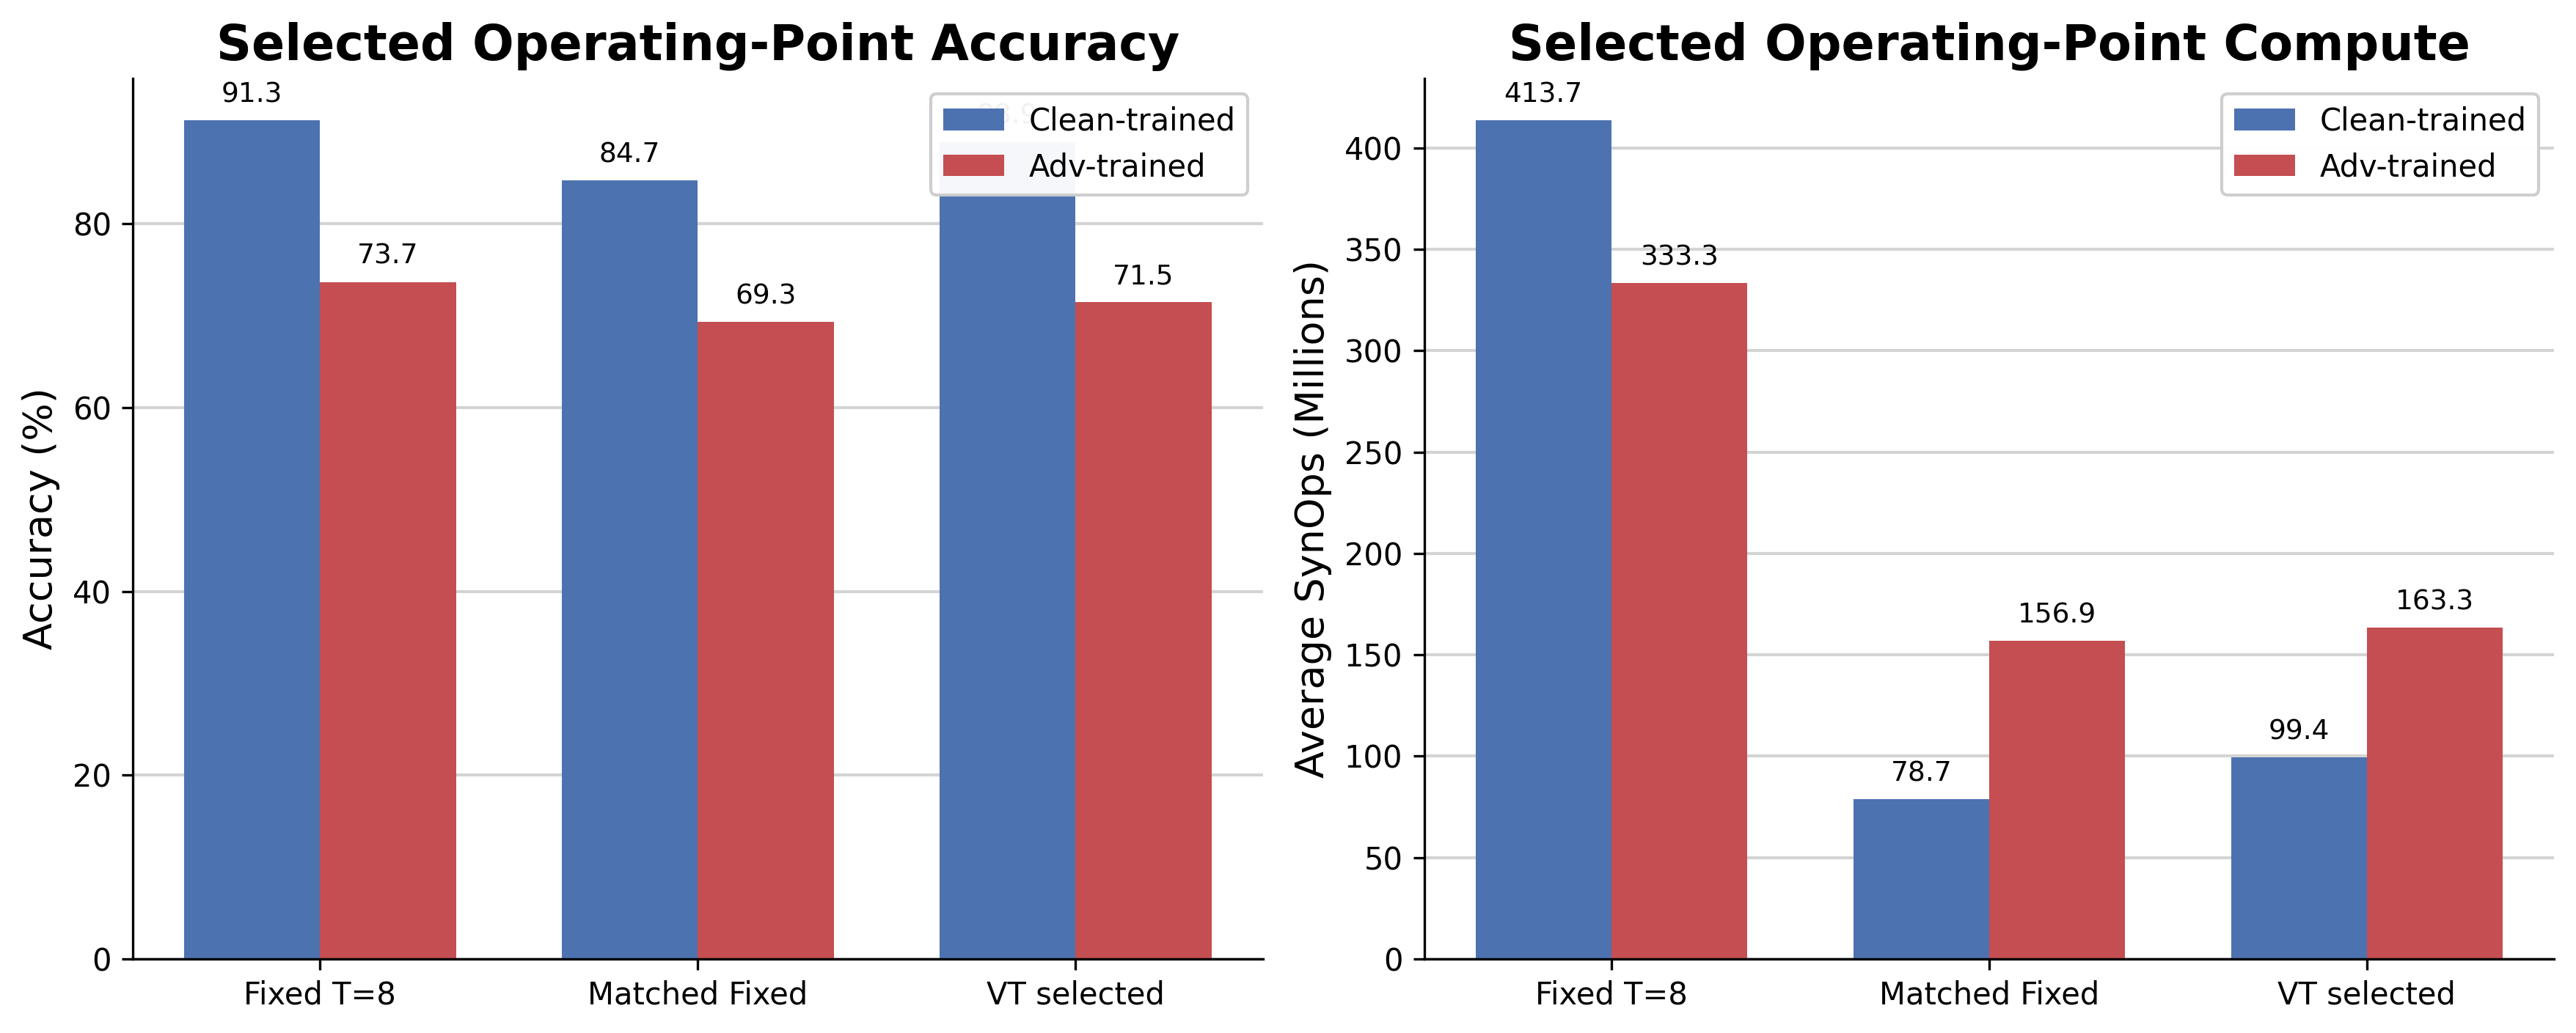
\includegraphics[width=\linewidth]{paper_figures/fig3_regime_selected_points.png}
\caption{Selected operating points under clean and adversarial training for the detailed ResNet case study. Each regime is summarized by full-horizon fixed inference, the clean-SynOps-matched fixed-time baseline, and the calibration-selected VT policy.}
\label{fig:selected-points}
\end{figure}

\begin{figure}[t]
\centering
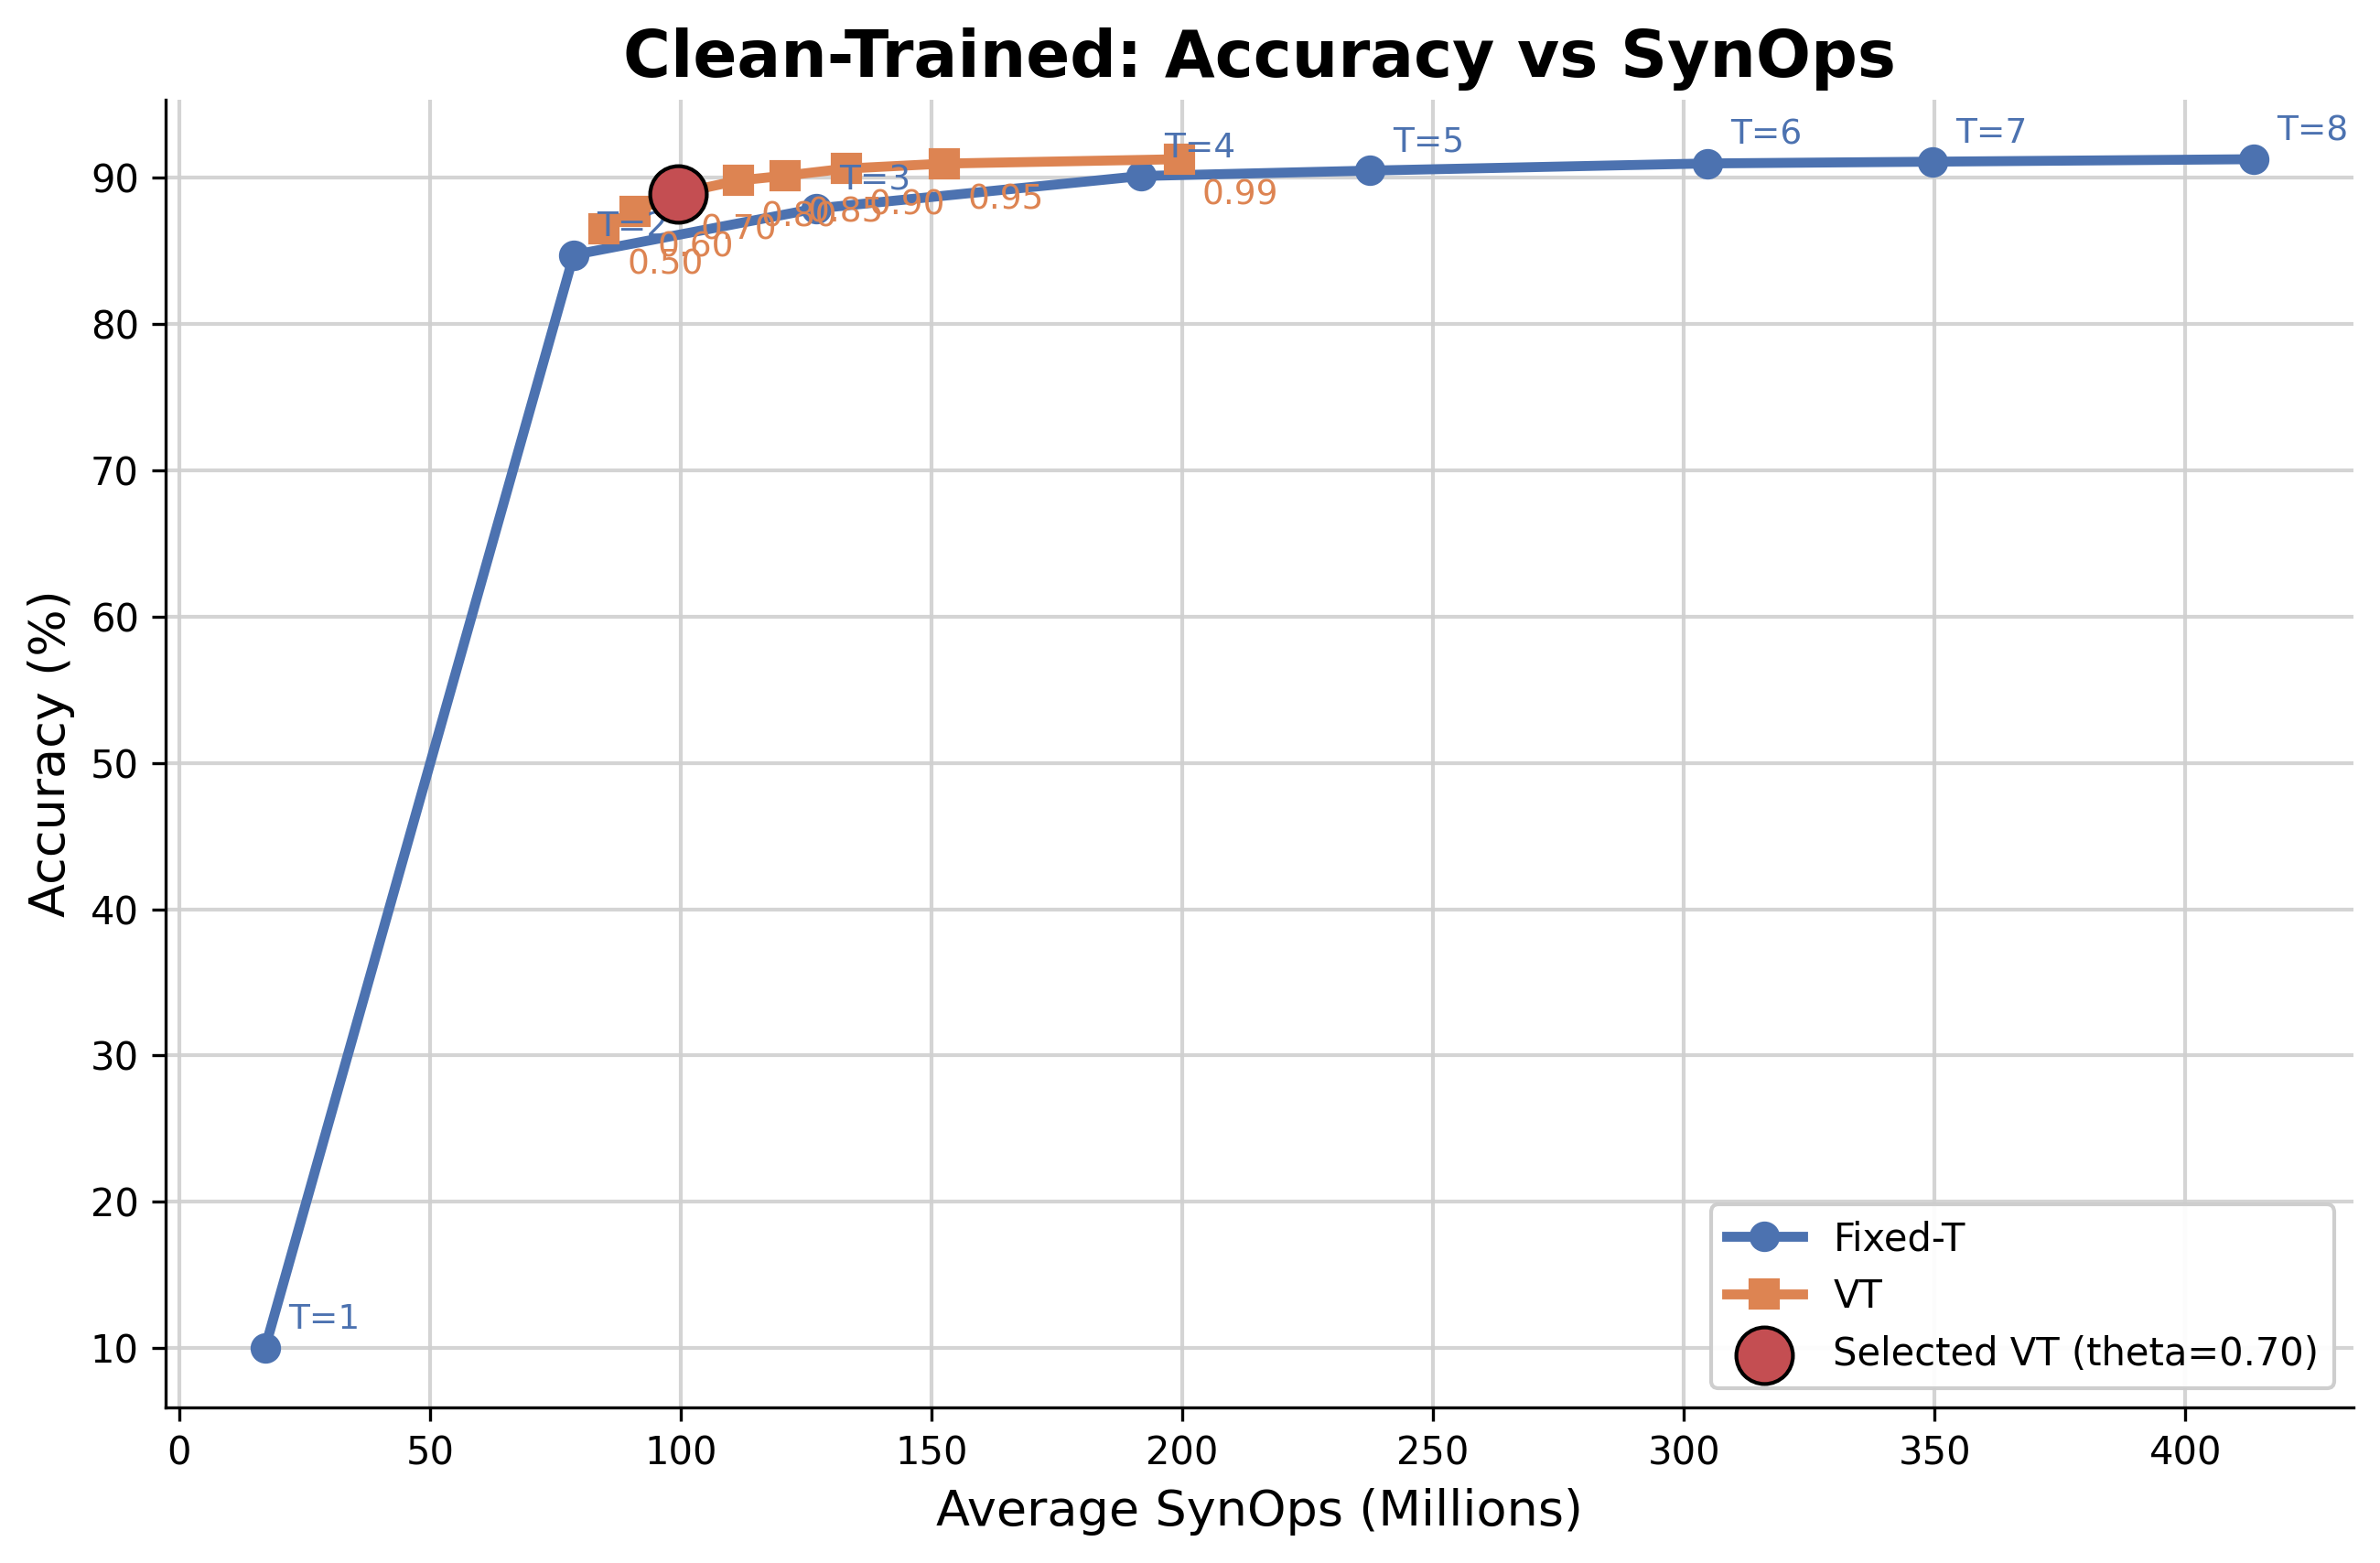
\includegraphics[width=0.92\linewidth]{paper_figures/fig_pareto_clean_accuracy_synops.png}
\caption{Clean-trained ResNet case study: direct accuracy--SynOps frontier for fixed-$T$ and VT operating points. The selected VT threshold lies well above the compute-matched fixed-time alternative.}
\label{fig:pareto-clean}
\end{figure}

\begin{figure}[t]
\centering
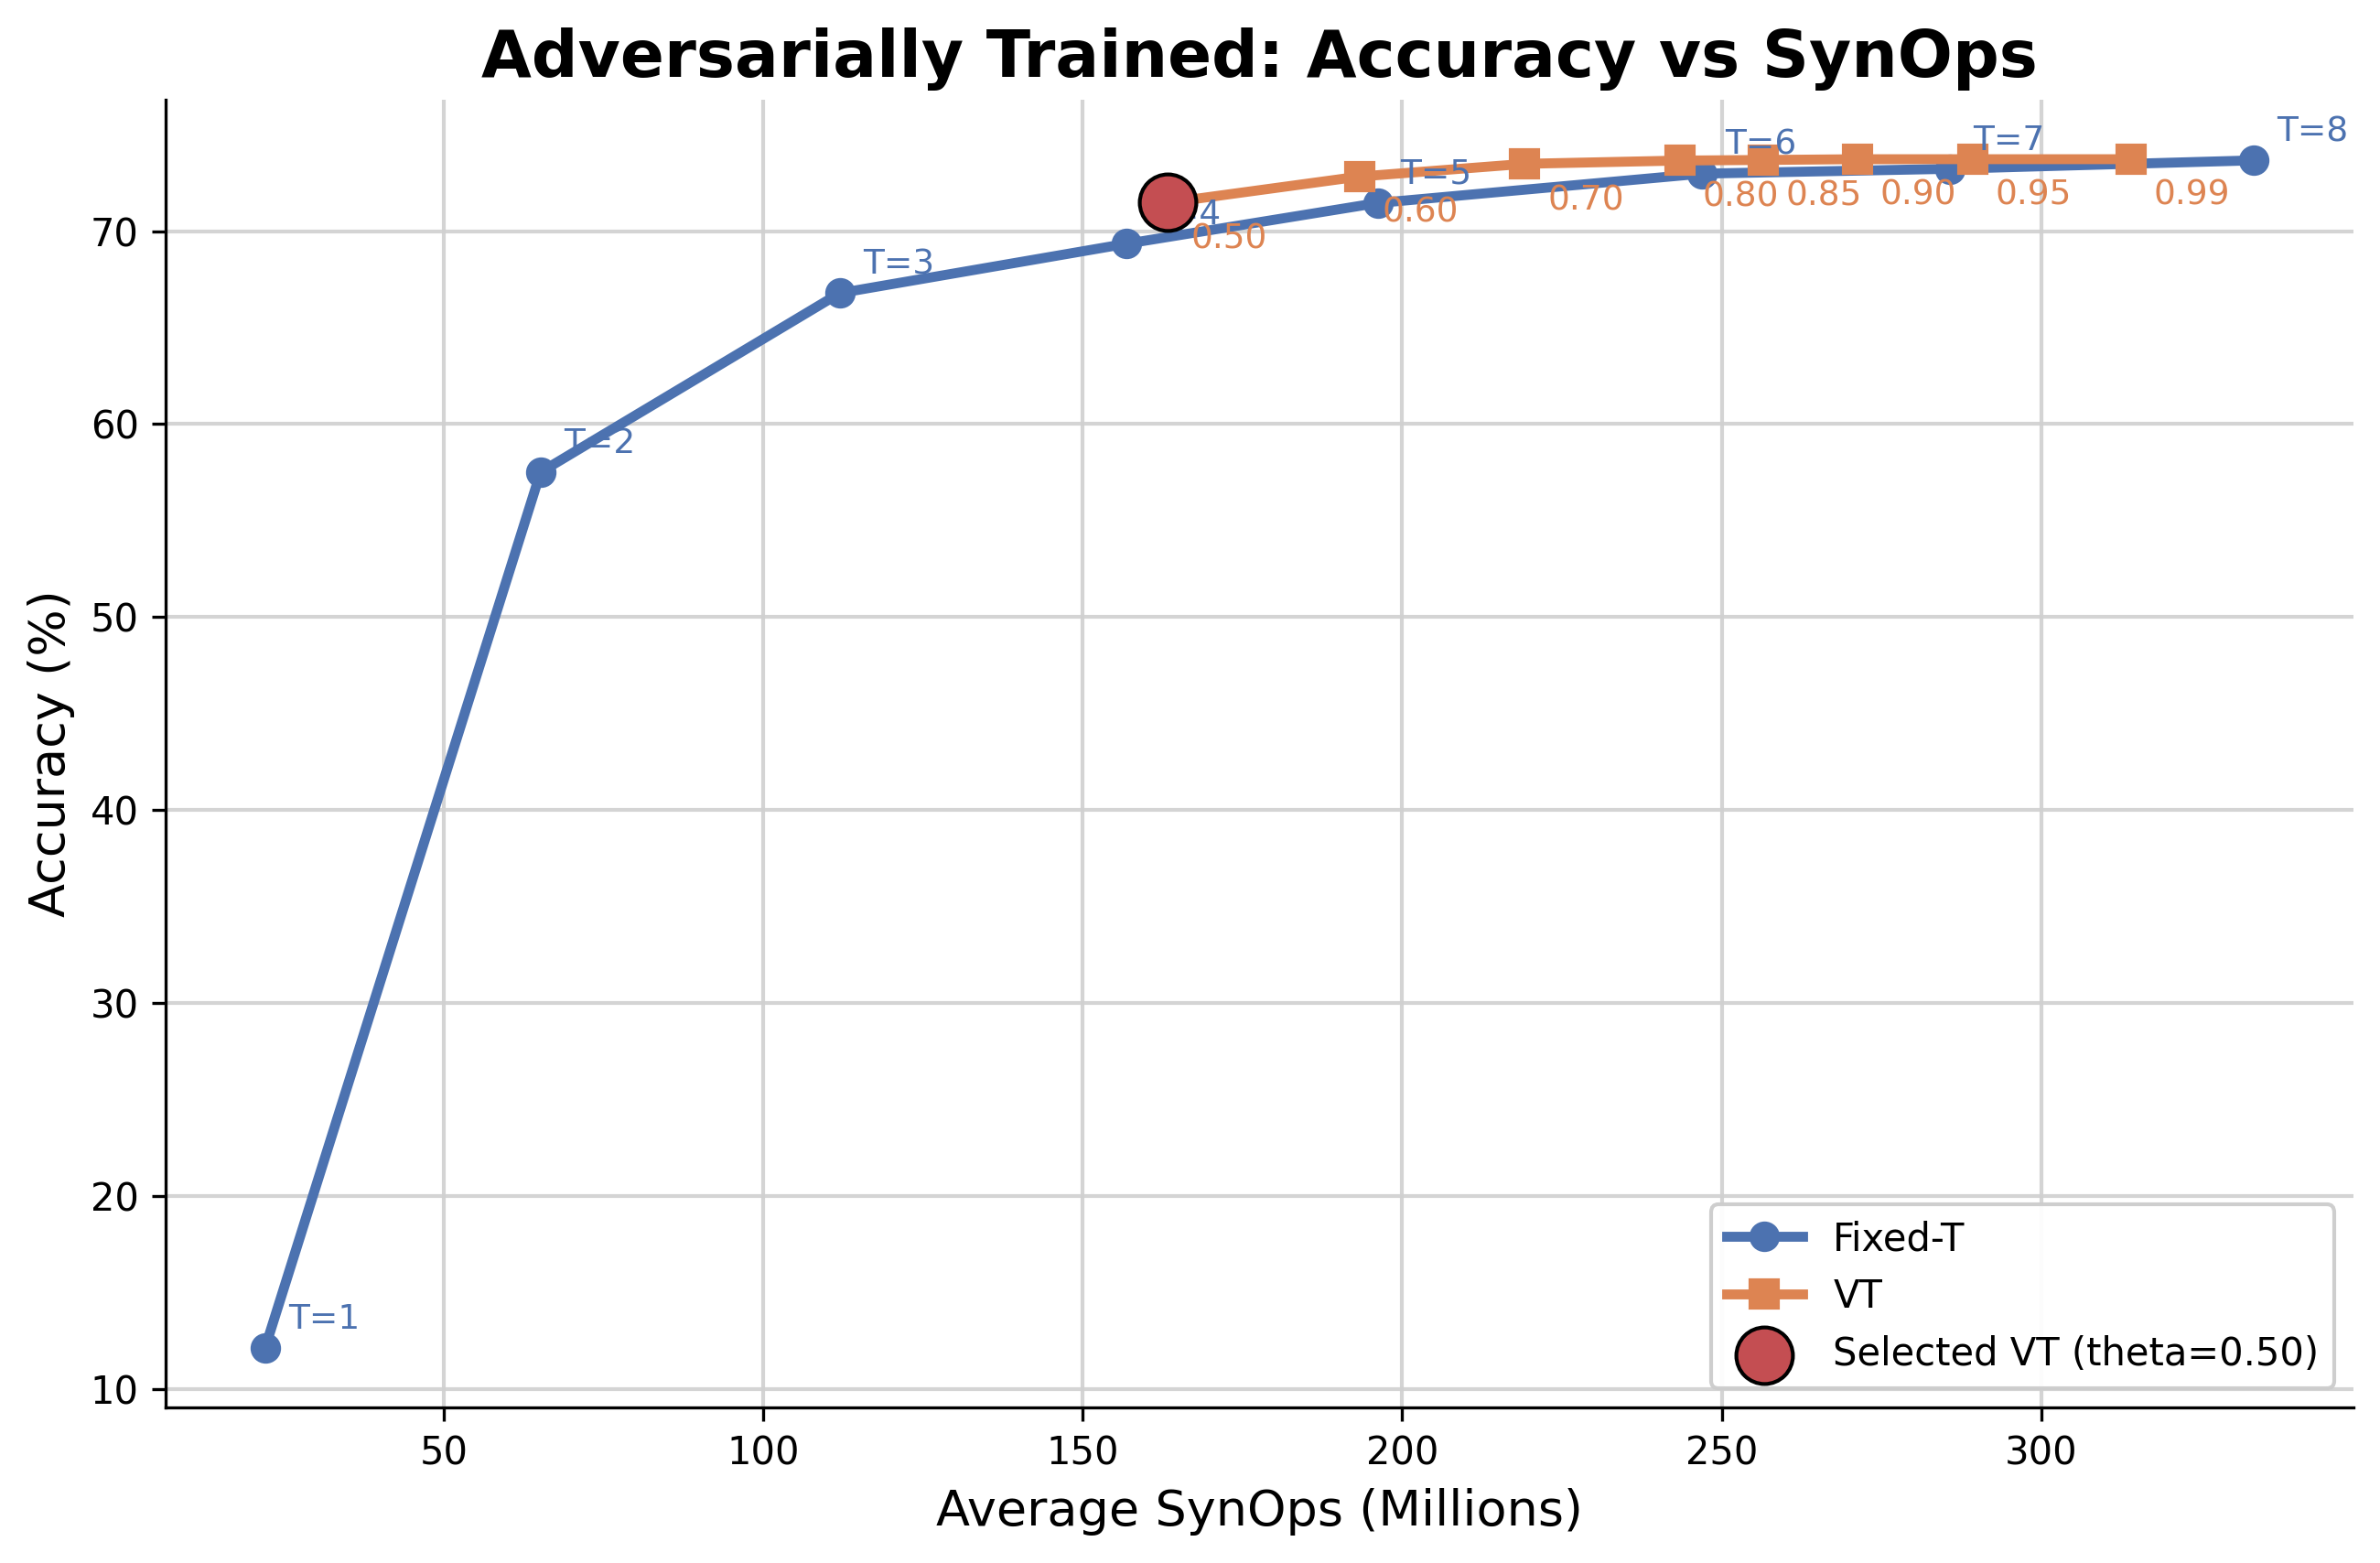
\includegraphics[width=0.92\linewidth]{paper_figures/fig_pareto_adv_accuracy_synops.png}
\caption{Adversarially trained ResNet case study: direct accuracy--SynOps frontier for fixed-$T$ and VT operating points. The VT advantage survives, but the frontier shifts inward relative to the clean-trained regime.}
\label{fig:pareto-adv}
\end{figure}

\subsection{Adversarial Training Alters VT Threshold Dynamics}
We next ask whether adversarial training simply lowers performance uniformly or whether it changes how VT behaves. The answer is that it changes the behavior materially on both backbones.

For ResNet, the clean-trained checkpoint selects $\theta=0.70$, stops on average at depth 2.393, and is matched to a very shallow fixed-time baseline ($T=2$). The adversarially trained checkpoint instead selects $\theta=0.50$, yet still stops much later on average, at depth 4.332, and is matched to $T=4$. VGG shows the same qualitative shift, but deeper overall: the clean-trained checkpoint selects $\theta=0.70$ at depth 3.533 and is matched to $T=3$, while the adversarially trained checkpoint selects $\theta=0.60$ at depth 6.272 and is matched to $T=6$. This indicates that adversarial training makes both backbones less willing to terminate early, with VGG already operating deeper than ResNet even before adversarial training. Figure~\ref{fig:regime-fixed-sweep} shows the detailed ResNet regime shift from the fixed-time side.

The relative VT gain also shrinks on both backbones. For ResNet, the compute-matched advantage drops from 4.19 points in the clean-trained case to 2.13 points in the adversarially trained case. For VGG, it drops from 6.49 points to 1.46 points. This implies that adversarial training compresses the clean VT benefit without eliminating it. However, it also shows that VT behavior cannot be understood without conditioning on the training regime.

\begin{figure}[t]
\centering
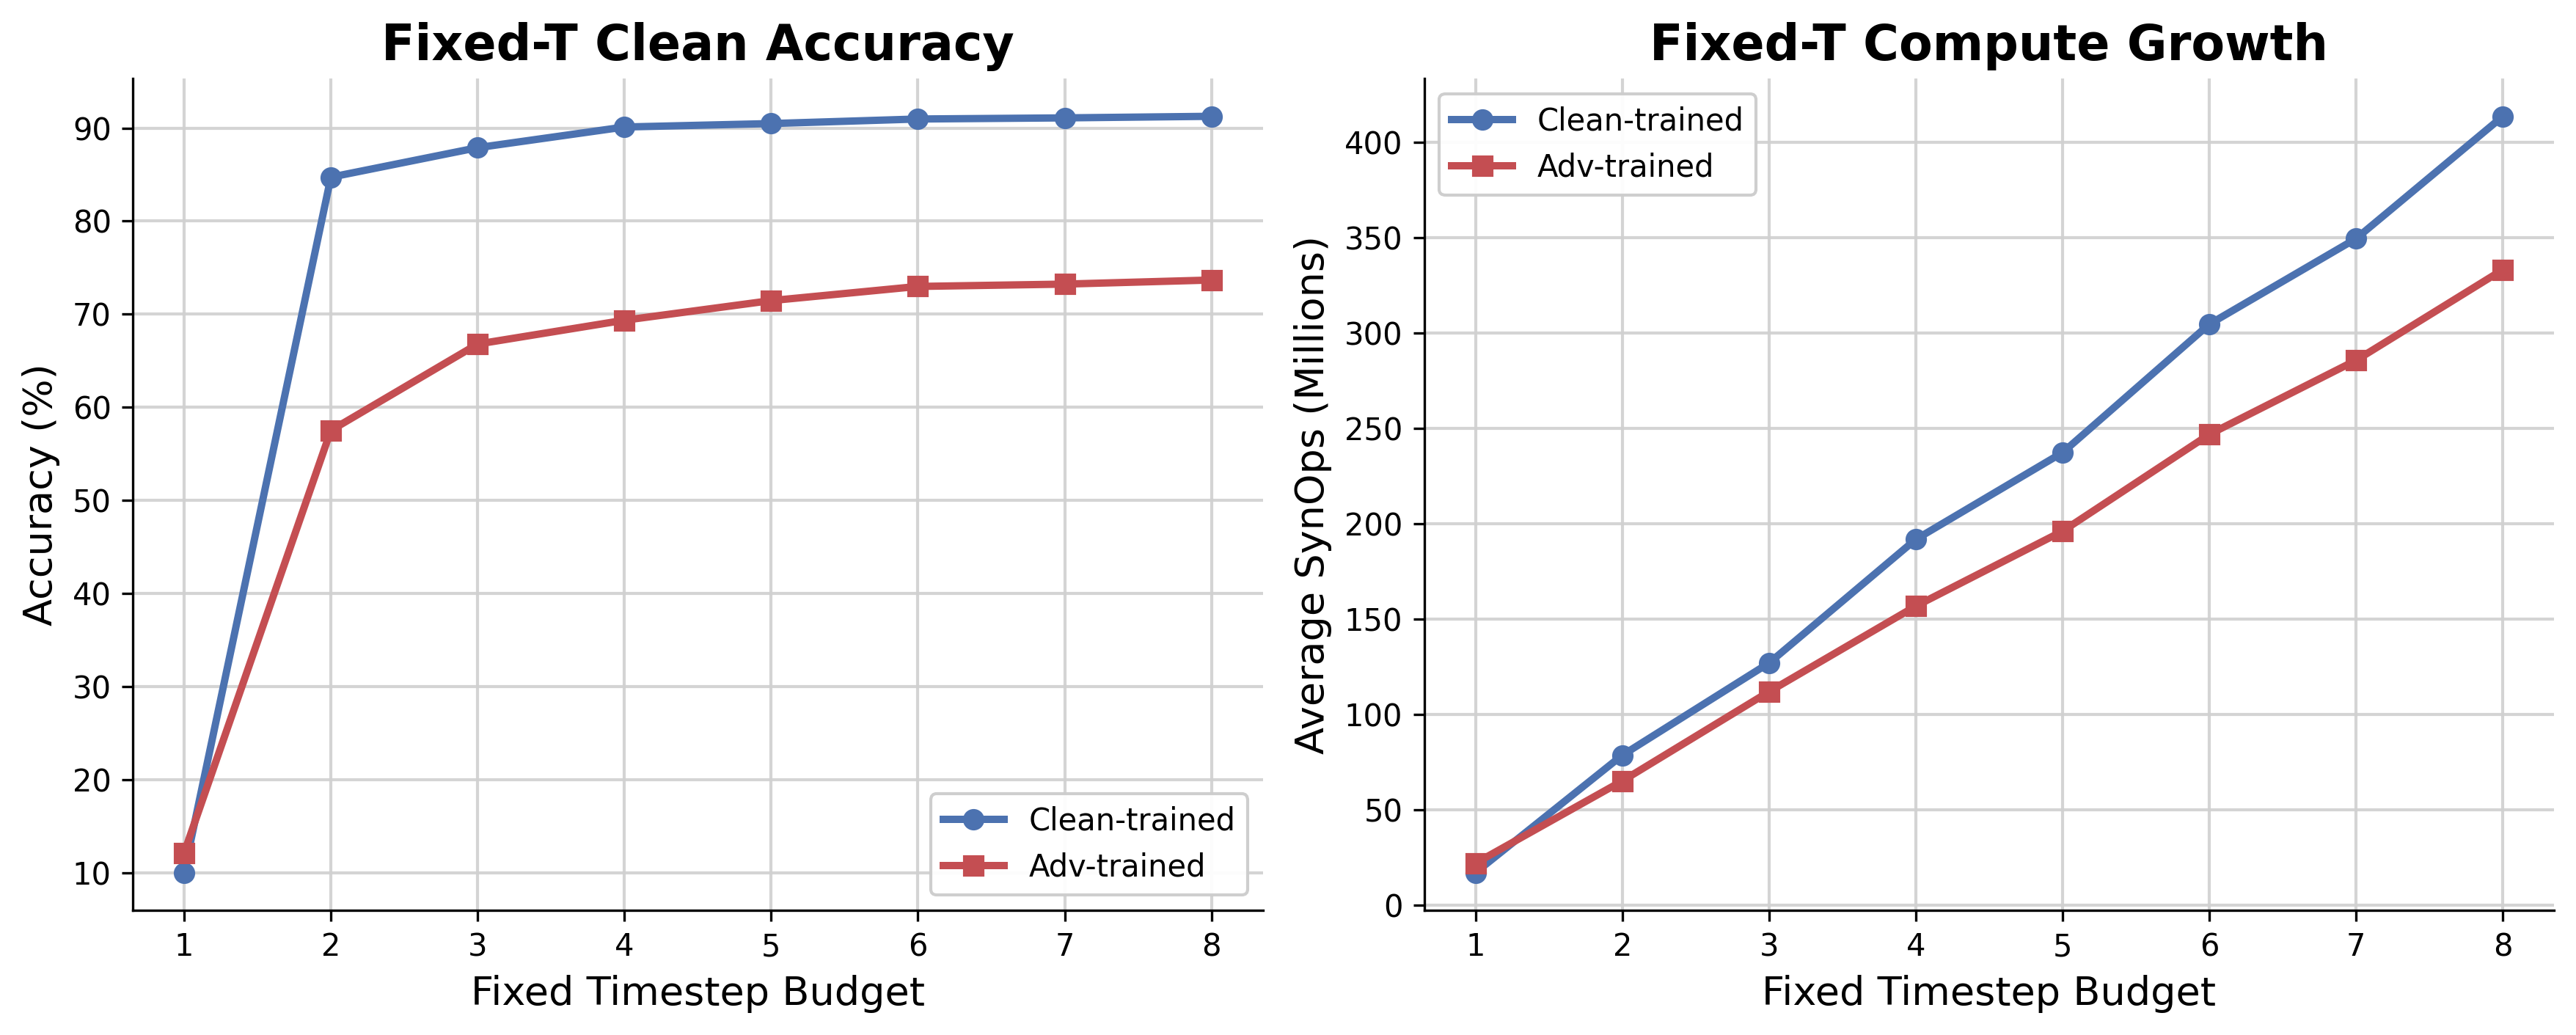
\includegraphics[width=\linewidth]{paper_figures/fig1_regime_fixed_t_sweep.png}
\caption{Cross-regime fixed-$T$ sweeps for the detailed ResNet case study. Adversarial training lowers the clean frontier and shifts the useful operating region toward deeper fixed horizons.}
\label{fig:regime-fixed-sweep}
\end{figure}

\subsection{The Clean VT Advantage Persists Beyond the Selected Threshold}
We then ask whether the selected threshold is a special case. The answer is no: the broader frontier supports the same conclusion.

For the clean-trained ResNet model, multiple thresholds beat compute-matched fixed-time baselines by large margins; for example, $\theta=0.60$ improves over matched $T=2$ by 3.00 points, while $\theta=0.95$ improves over matched $T=3$ by 3.07 points. At $\theta=0.99$, VT matches full-horizon clean accuracy while still using much less compute than fixed $T=8$. Clean-trained VGG shows the same behavior with even larger gains at the selected point: $\theta=0.70$ improves over matched $T=3$ by 6.49 points, and neighboring thresholds from 0.60 to 0.90 also outperform their compute-matched fixed controls by more than three points.

For the adversarially trained ResNet model, the frontier is similarly smooth. Although $\theta=0.50$ is the calibration-selected point, higher thresholds nearly recover full-horizon clean accuracy. In particular, $\theta=0.70$ reaches \SI{73.49}{\percent}, essentially matching full $T=8$ accuracy at substantially lower average depth. Adversarially trained VGG shows a shallower advantage, but the same frontier shape: $\theta=0.60$ is selected on calibration, higher thresholds approach the full-horizon clean accuracy, and VT remains above matched fixed-time truncation across the main part of the frontier. This implies that adversarial training shifts the VT frontier rather than destroying it. However, the calibration-selected point remains the fairest headline result because it was not chosen on the test set. Figure~\ref{fig:regime-vt-sweep} shows this directly for the ResNet case study.

\begin{figure}[t]
\centering
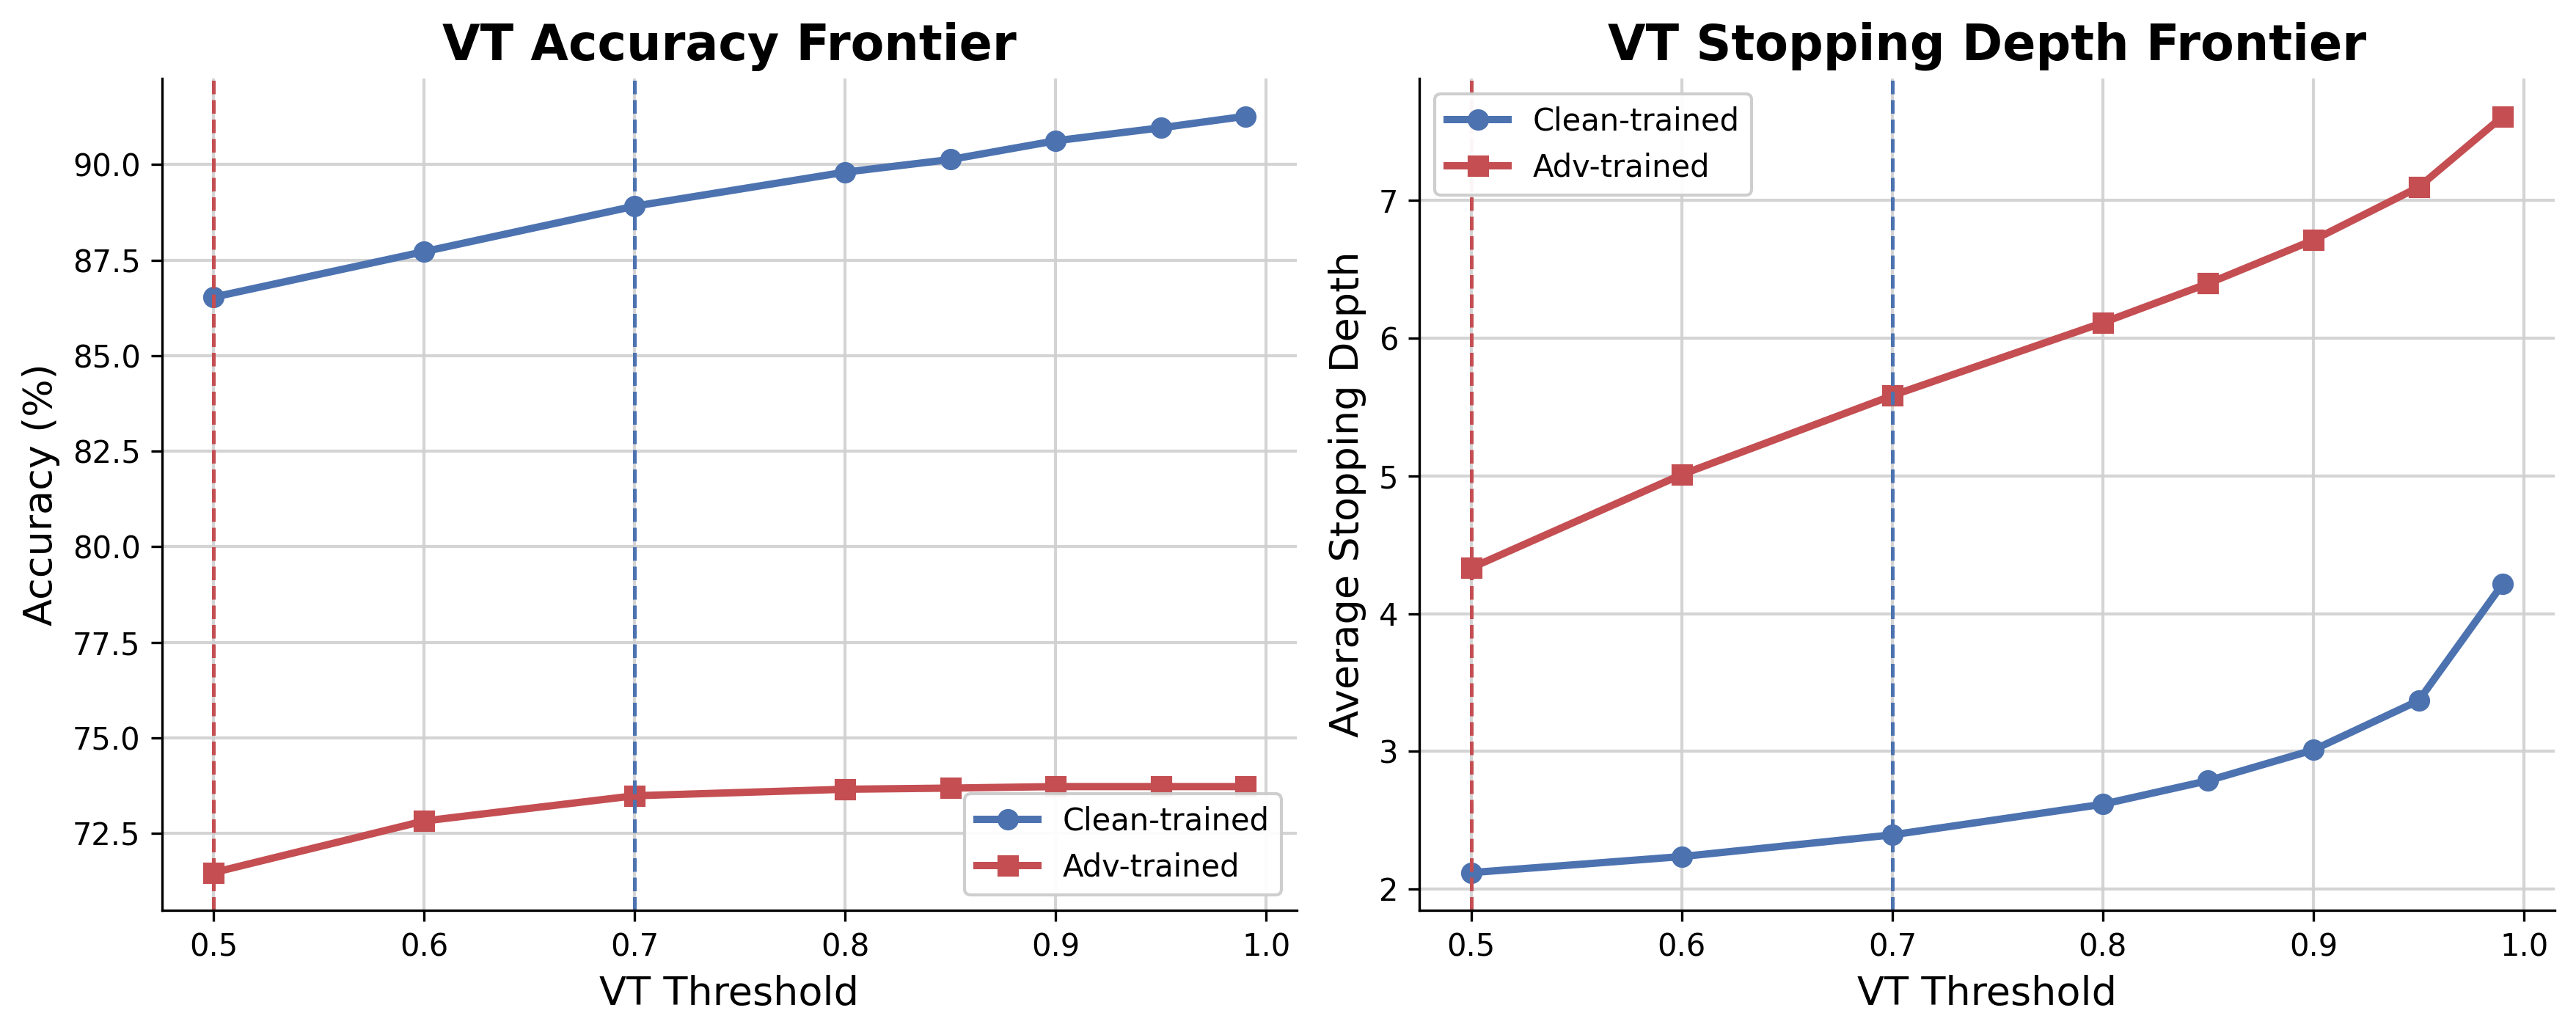
\includegraphics[width=\linewidth]{paper_figures/fig2_regime_vt_threshold_sweep.png}
\caption{Cross-regime VT threshold sweeps for the detailed ResNet case study. Adversarial training shifts both the accuracy frontier and the stopping-depth frontier, but VT remains effective over a broad range of thresholds.}
\label{fig:regime-vt-sweep}
\end{figure}

\subsection{Clean Efficiency Gains Generalize Across Stopping Rules}
We next ask whether the main result depends on one particular stopping heuristic. The answer is largely no.

Table~\ref{tab:stopping_rules} shows that the broad pattern is stable across both regimes on the detailed ResNet case study, and VGG follows the same qualitative ordering. On clean-trained VGG, \texttt{max\_softmax} and \texttt{margin} tie at \SI{86.99}{\percent}, while \texttt{temperature\_softmax} reaches \SI{87.39}{\percent} at higher compute. On adversarially trained VGG, \texttt{temperature\_softmax} slightly edges out \texttt{max\_softmax} in clean accuracy, but the differences remain small and do not change the main selected-point story.

This implies that the main VT effect is not a fragile artifact of one stopping rule. However, max-softmax remains the most natural default because it is simple, standard, and already strong enough to support the central claim. Figure~\ref{fig:regime-stop-rules} makes the regime comparison explicit: the relative ranking of rules is stable, but the adversarially trained model pays a clear accuracy and depth penalty overall.

\begin{table}[t]
\centering
\caption{Stopping-rule comparison on the test set.}
\label{tab:stopping_rules}
\begin{tabular}{llccc}
\toprule
Regime & Rule & Threshold & Accuracy (\%) & Avg. Depth \\
\midrule
\multirow{6}{*}{Clean-trained}
& Fixed $T=8$ & -- & 91.26 & 8.000 \\
& Max-softmax & 0.70 & 88.91 & 2.393 \\
& Margin & 0.50 & 89.04 & 2.378 \\
& Entropy & 0.60 & 88.14 & 2.344 \\
& Temp.-softmax & 0.50 & 89.35 & 2.586 \\
& Evidential surrogate & 0.50 & 86.38 & 2.195 \\
\midrule
\multirow{6}{*}{Adv.-trained}
& Fixed $T=8$ & -- & 73.67 & 8.000 \\
& Max-softmax & 0.50 & 71.48 & 4.332 \\
& Margin & 0.50 & 73.31 & 5.425 \\
& Entropy & 0.50 & 72.24 & 4.998 \\
& Temp.-softmax & 0.50 & 73.61 & 6.157 \\
& Evidential surrogate & 0.50 & 67.99 & 3.748 \\
\bottomrule
\end{tabular}
\end{table}

\begin{figure}[t]
\centering
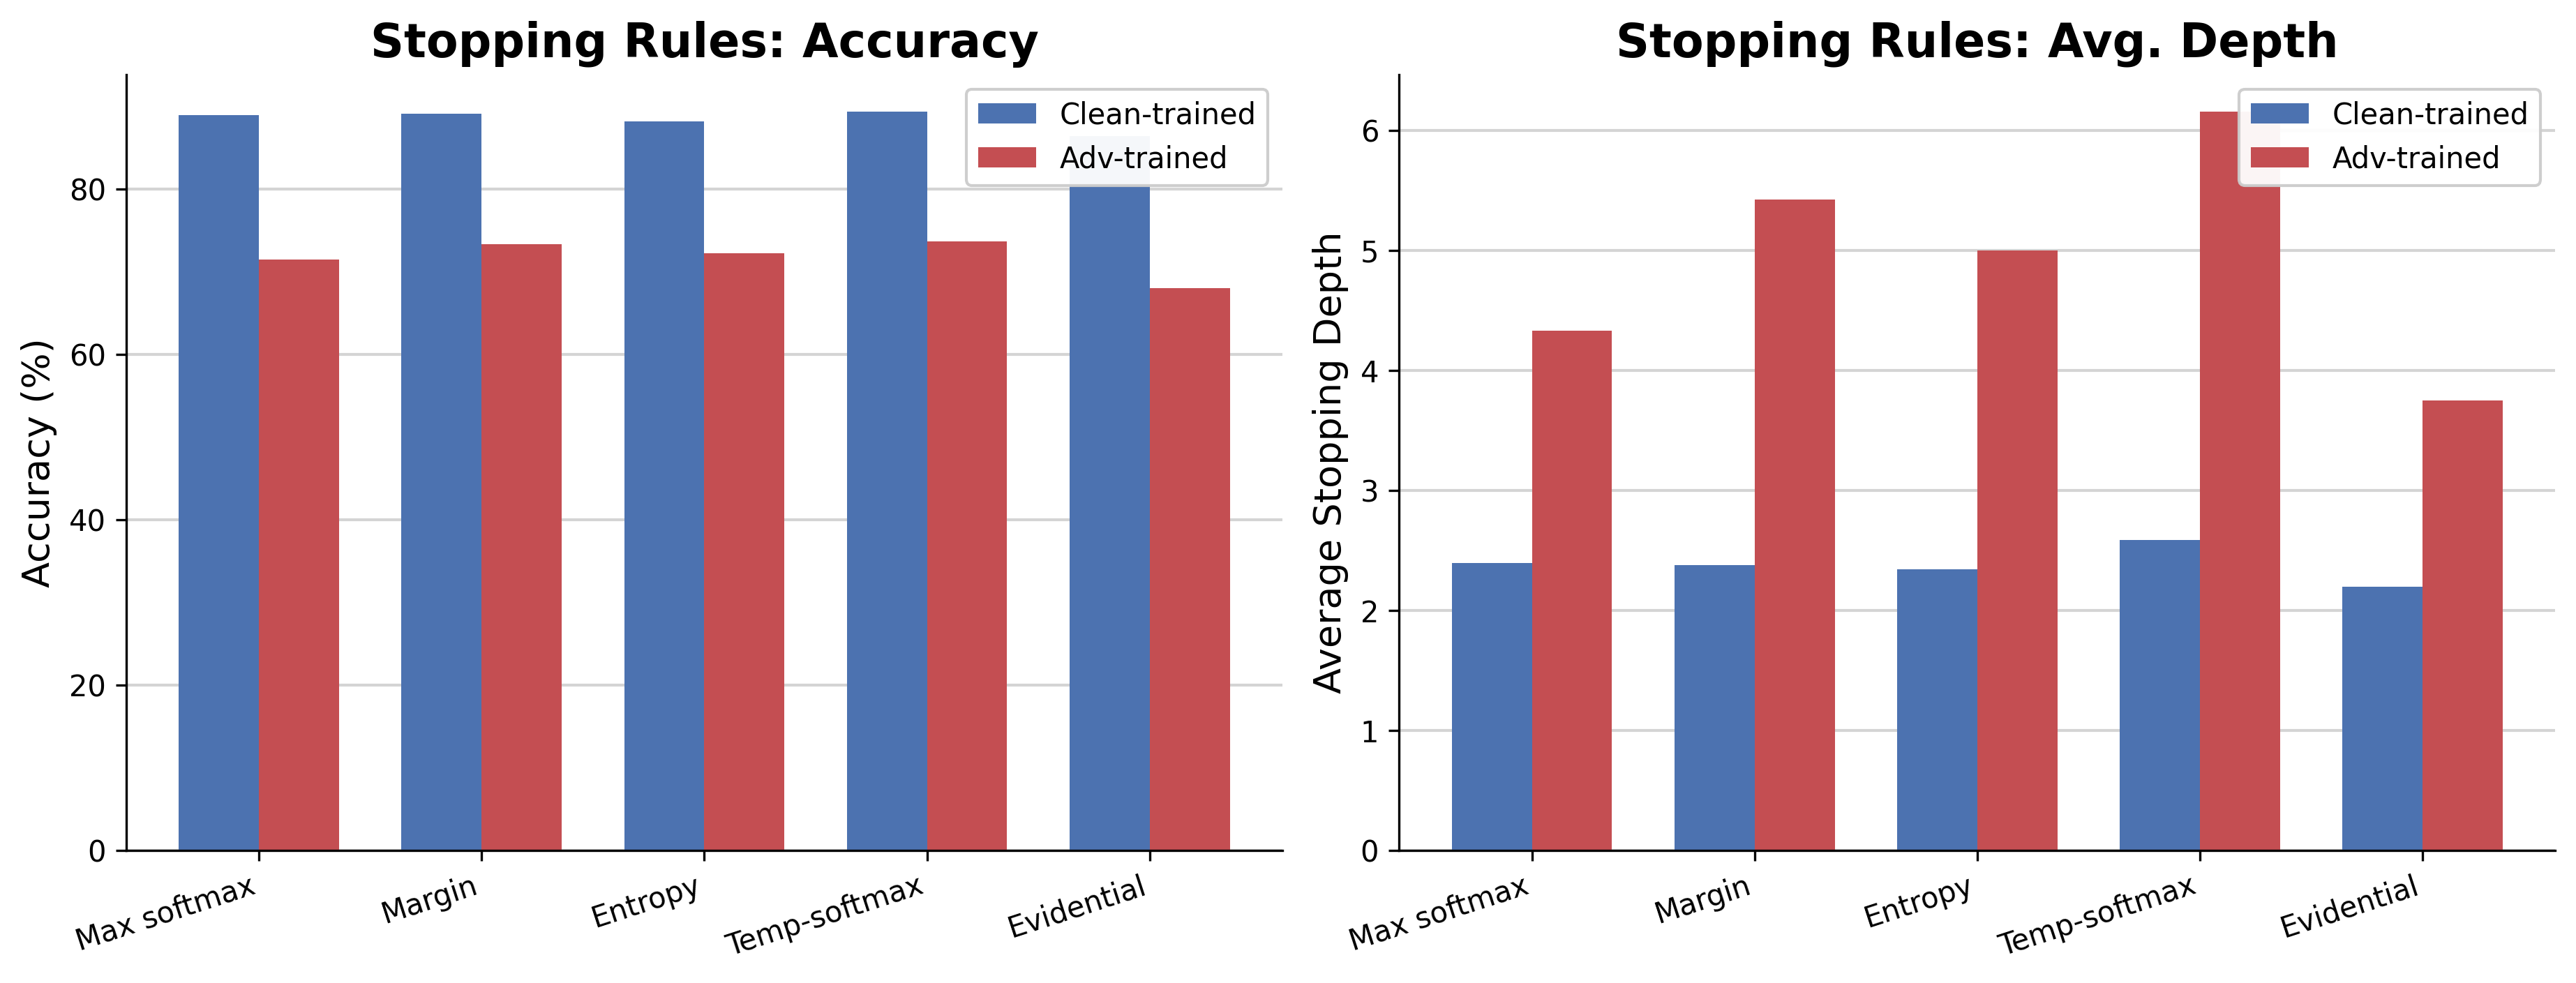
\includegraphics[width=\linewidth]{paper_figures/fig4_regime_stopping_rules.png}
\caption{Stopping-rule comparison across training regimes for the detailed ResNet case study. The broad rule ordering is stable, but adversarial training lowers clean accuracy and generally requires deeper inference.}
\label{fig:regime-stop-rules}
\end{figure}

\subsection{Deterministic VT Introduces Adversarial Vulnerabilities}
We then ask whether the clean VT benefit extends from efficiency to adversarial robustness. The answer is not clearly.

For the clean-trained checkpoints, the answer is simple: it does not. On both ResNet and VGG, untargeted PGD-20 reduces fixed $T=8$ and selected VT to approximately zero robust accuracy, and AutoAttack reaches the same conclusion. This implies that strong clean efficiency gains do not tell us anything positive about robustness on a clean-trained backbone.

For the adversarially trained checkpoints, the fairest question is not only how VT compares with full $T=8$, but how it compares with the \emph{compute-matched fixed-time control}. On ResNet, clean-side SynOps matching maps the selected VT threshold $\theta=0.50$ to fixed $T=4$. On a class-balanced \num{1000}-sample subset, the resulting three-way comparison is mixed but revealing: under PGD, fixed $T=8$ reaches \SI{44.1}{\percent}, selected VT reaches \SI{43.1}{\percent}, and the matched fixed-$T=4$ control reaches \SI{40.2}{\percent}. Under AutoAttack, however, the ranking reverses sharply: the matched fixed-$T=4$ control reaches \SI{33.7}{\percent}, fixed $T=8$ reaches \SI{22.2}{\percent}, and selected VT falls to only \SI{10.5}{\percent}. VGG provides a second-backbone check on the same phenomenon. There, clean-side SynOps matching maps the selected threshold $\theta=0.60$ to fixed $T=6$. On the matched \num{1000}-sample subset, PGD gives \SI{45.2}{\percent} for fixed $T=8$, \SI{41.7}{\percent} for matched fixed $T=6$, and \SI{45.9}{\percent} for selected VT, while AutoAttack gives \SI{9.7}{\percent}, \SI{20.2}{\percent}, and \SI{8.2}{\percent}, respectively.

This subset-aligned result is the paper's strongest cautionary evidence. On both backbones, VT can still look competitive under PGD when compared against both full $T=8$ and its matched fixed-time control, yet become decisively worse than the matched fixed baseline under AutoAttack. A full fixed-$T$ sweep on the same subset sharpens the point further for ResNet. Under PGD, the best fixed-time operating point is indeed the full-horizon model ($T=8$, \SI{44.1}{\percent}), while VT thresholds $\theta=0.60$ and $\theta=0.70$ reach \SI{44.3}{\percent} and \SI{44.7}{\percent}, respectively. Under AutoAttack, however, the robust fixed-time optimum shifts dramatically earlier: $T=2$ reaches \SI{35.7}{\percent} and $T=3$ reaches \SI{35.0}{\percent}, whereas the best VT threshold we tested, $\theta=0.70$, reaches only \SI{20.3}{\percent}. Figure~\ref{fig:attack-sweep-standalone} visualizes this reviewer-critical ResNet sweep directly. Read together with the full-test results, the message is consistent: on the full \num{10000}-sample test set, adversarially trained ResNet reaches \SI{23.12}{\percent} for selected VT versus \SI{20.96}{\percent} for fixed $T=8$ under PGD and \SI{4.14}{\percent} versus \SI{7.57}{\percent} under AutoAttack, while adversarially trained VGG reaches \SI{44.45}{\percent} versus \SI{45.90}{\percent} under PGD and \SI{8.55}{\percent} versus \SI{10.75}{\percent} under AutoAttack. Thus, the mild PGD competitiveness does not survive the stronger robustness test.

The implication is not that VT is uniformly harmful, but that its clean advantage does not automatically survive the fair robustness comparison that matters most. Deterministic VT appears to expose an attack surface that is only partly visible under PGD and becomes much clearer under AutoAttack. The fixed-$T$ sweep also shows that the ``right'' robustness baseline is attack-dependent: under strong attack, the best fixed-time deployment may be a short horizon rather than full $T=8$. Because the matched-control and fixed-$T$ sweep robustness checks are currently subset-based rather than full-test, we present them as strong supporting evidence rather than the final definitive robustness table. Figure~\ref{fig:regime-robustness} collects the full-test and subset-aligned robustness comparisons in one place.

\begin{table}[t]
\centering
\caption{Robustness summary for the selected VT operating point on both backbones.}
\label{tab:robustness}
\begin{tabular}{lllcc}
\toprule
Backbone & Regime & Attack & Fixed $T=8$ (\%) & VT Selected (\%) \\
\midrule
\multirow{4}{*}{ResNet-18} & Clean-trained & PGD-20 untargeted & 0.00 & 0.02 \\
 & Clean-trained & AutoAttack & 0.06 & 0.02 \\
 & Adv.-trained & PGD-20 untargeted & 20.96 & 23.12 \\
 & Adv.-trained & AutoAttack & 7.57 & 4.14 \\
\midrule
\multirow{4}{*}{VGG16} & Clean-trained & PGD-20 untargeted & 0.05 & 0.10 \\
 & Clean-trained & AutoAttack & 0.00 & 0.00 \\
 & Adv.-trained & PGD-20 untargeted & 45.90 & 44.45 \\
 & Adv.-trained & AutoAttack & 10.75 & 8.55 \\
\bottomrule
\end{tabular}
\end{table}

\begin{figure}[t]
\centering
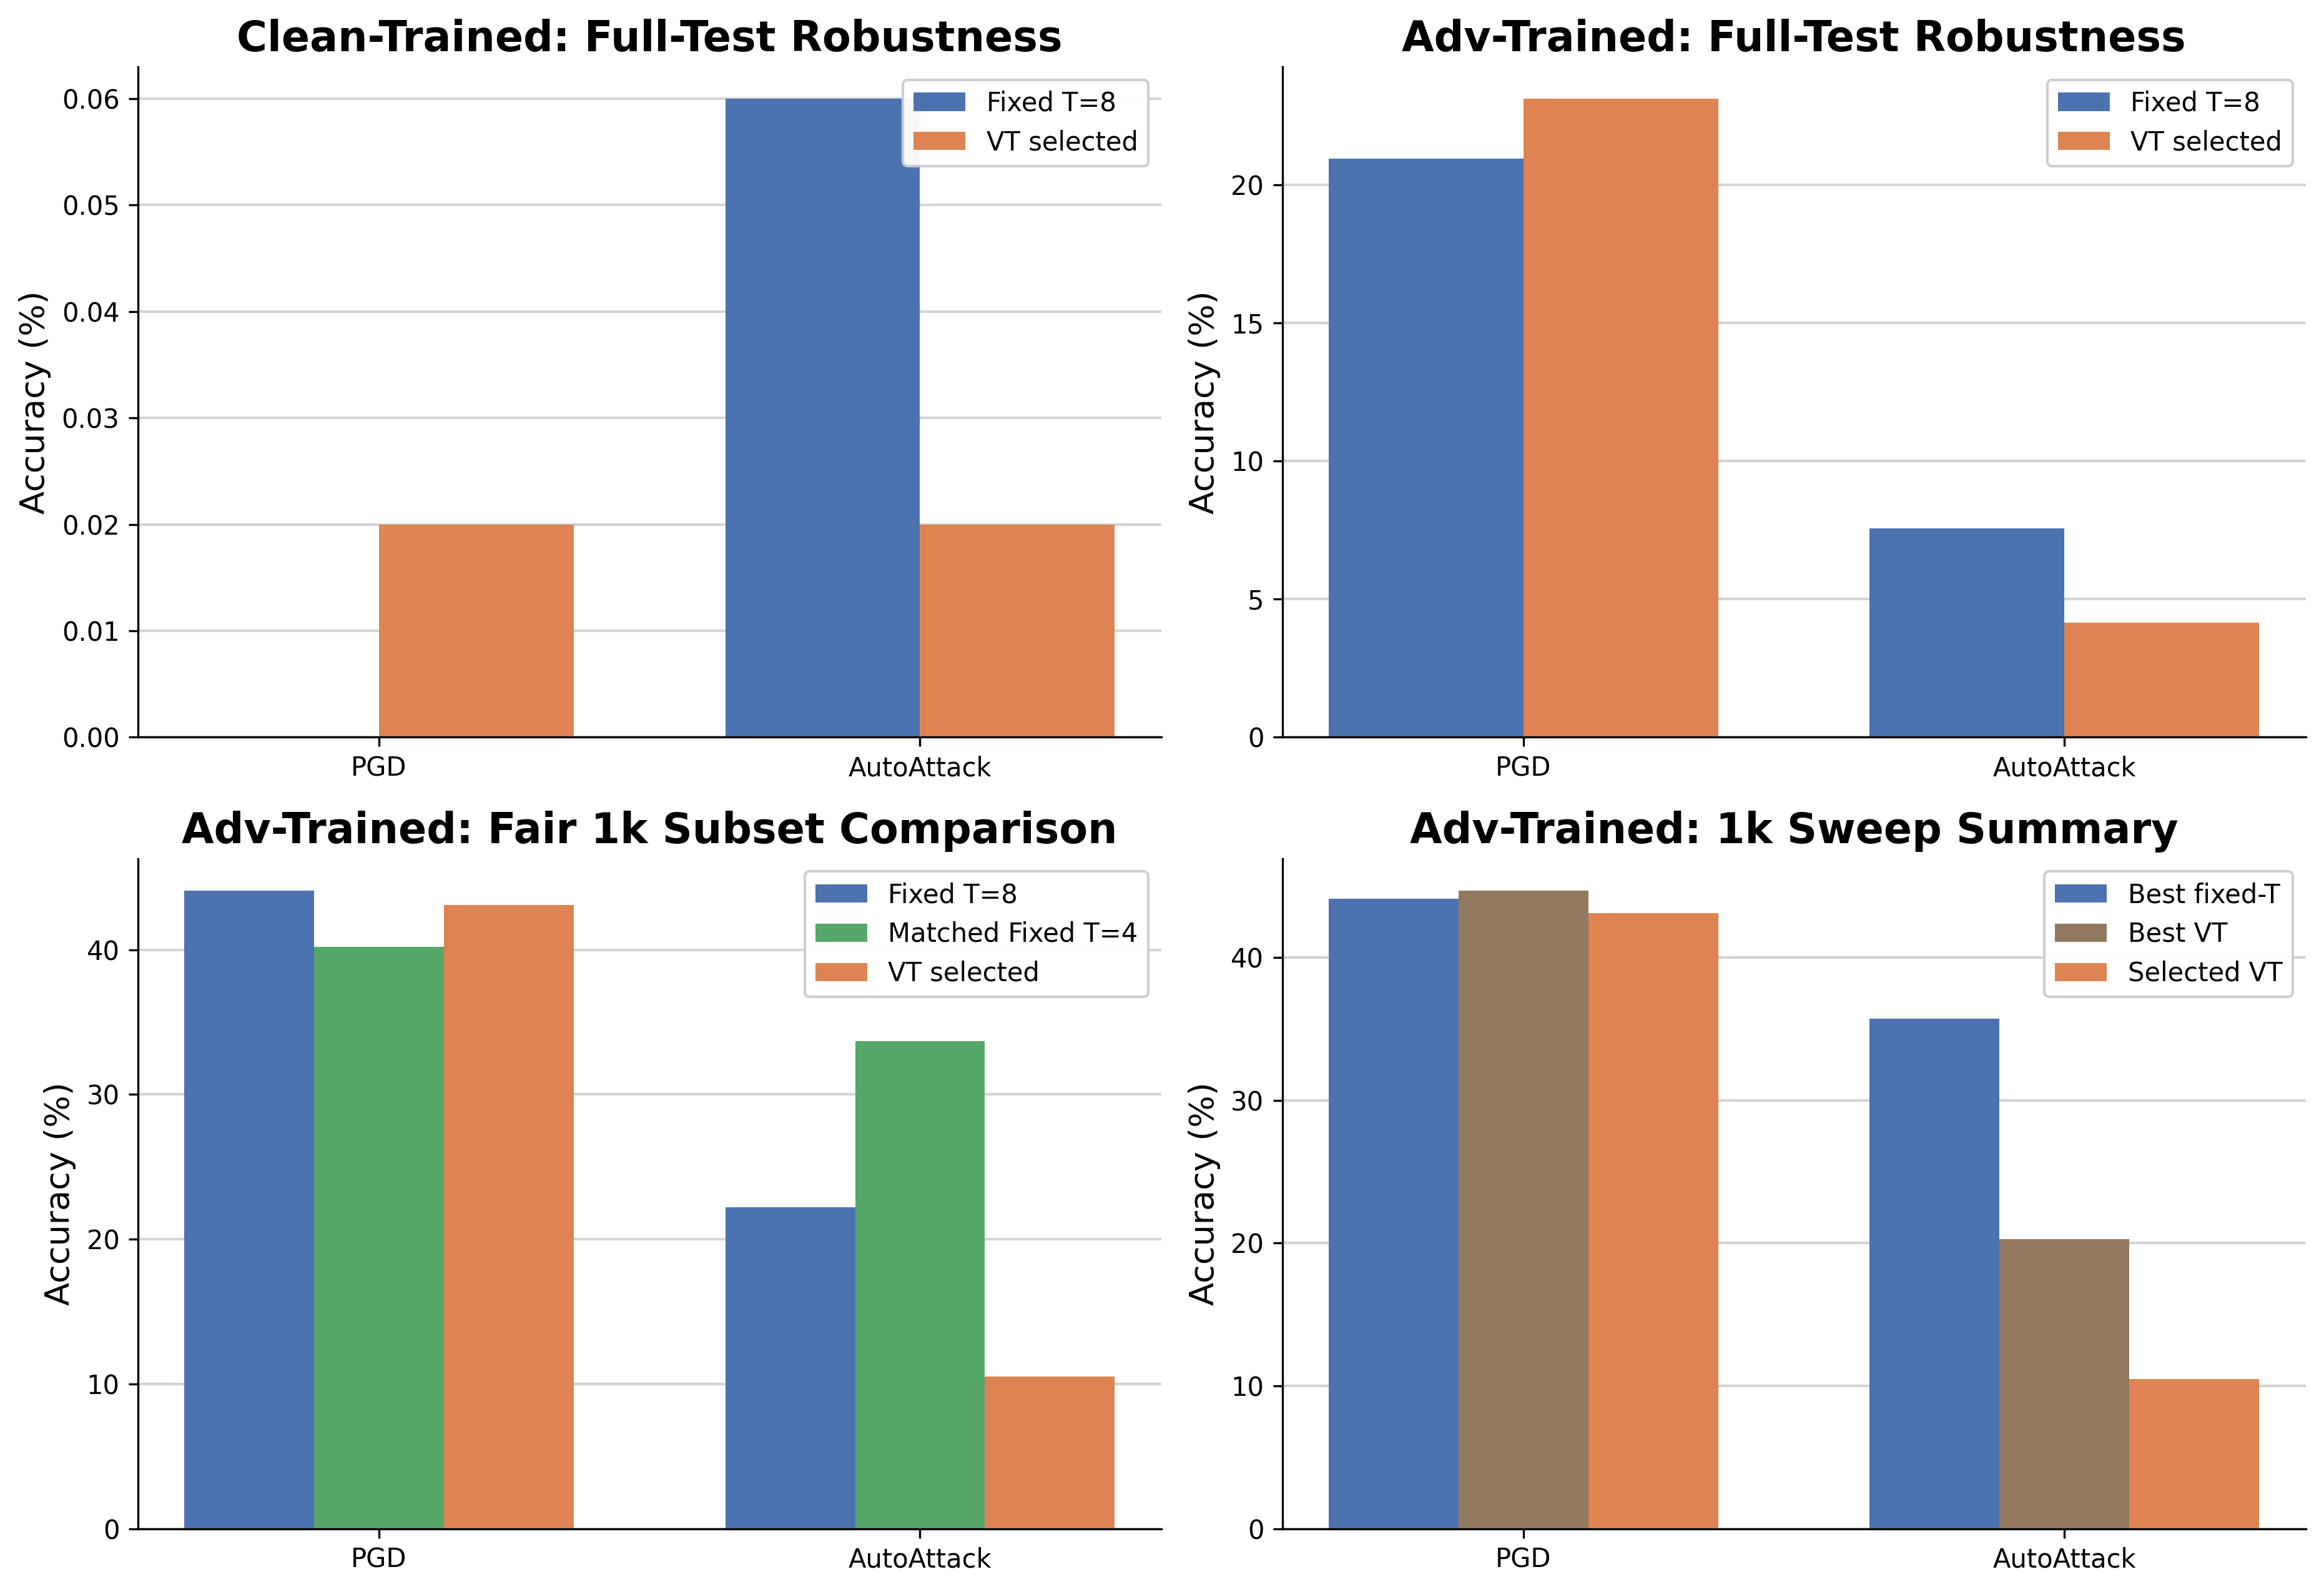
\includegraphics[width=\linewidth]{paper_figures/fig5_regime_robustness.png}
\caption{Robustness comparisons across regimes and evaluation scopes for the detailed ResNet case study. The top row shows the full-test selected-point results, while the bottom row shows the adversarial-trained subset fairness check and the subset attack sweep summary.}
\label{fig:regime-robustness}
\end{figure}

\begin{figure}[t]
\centering
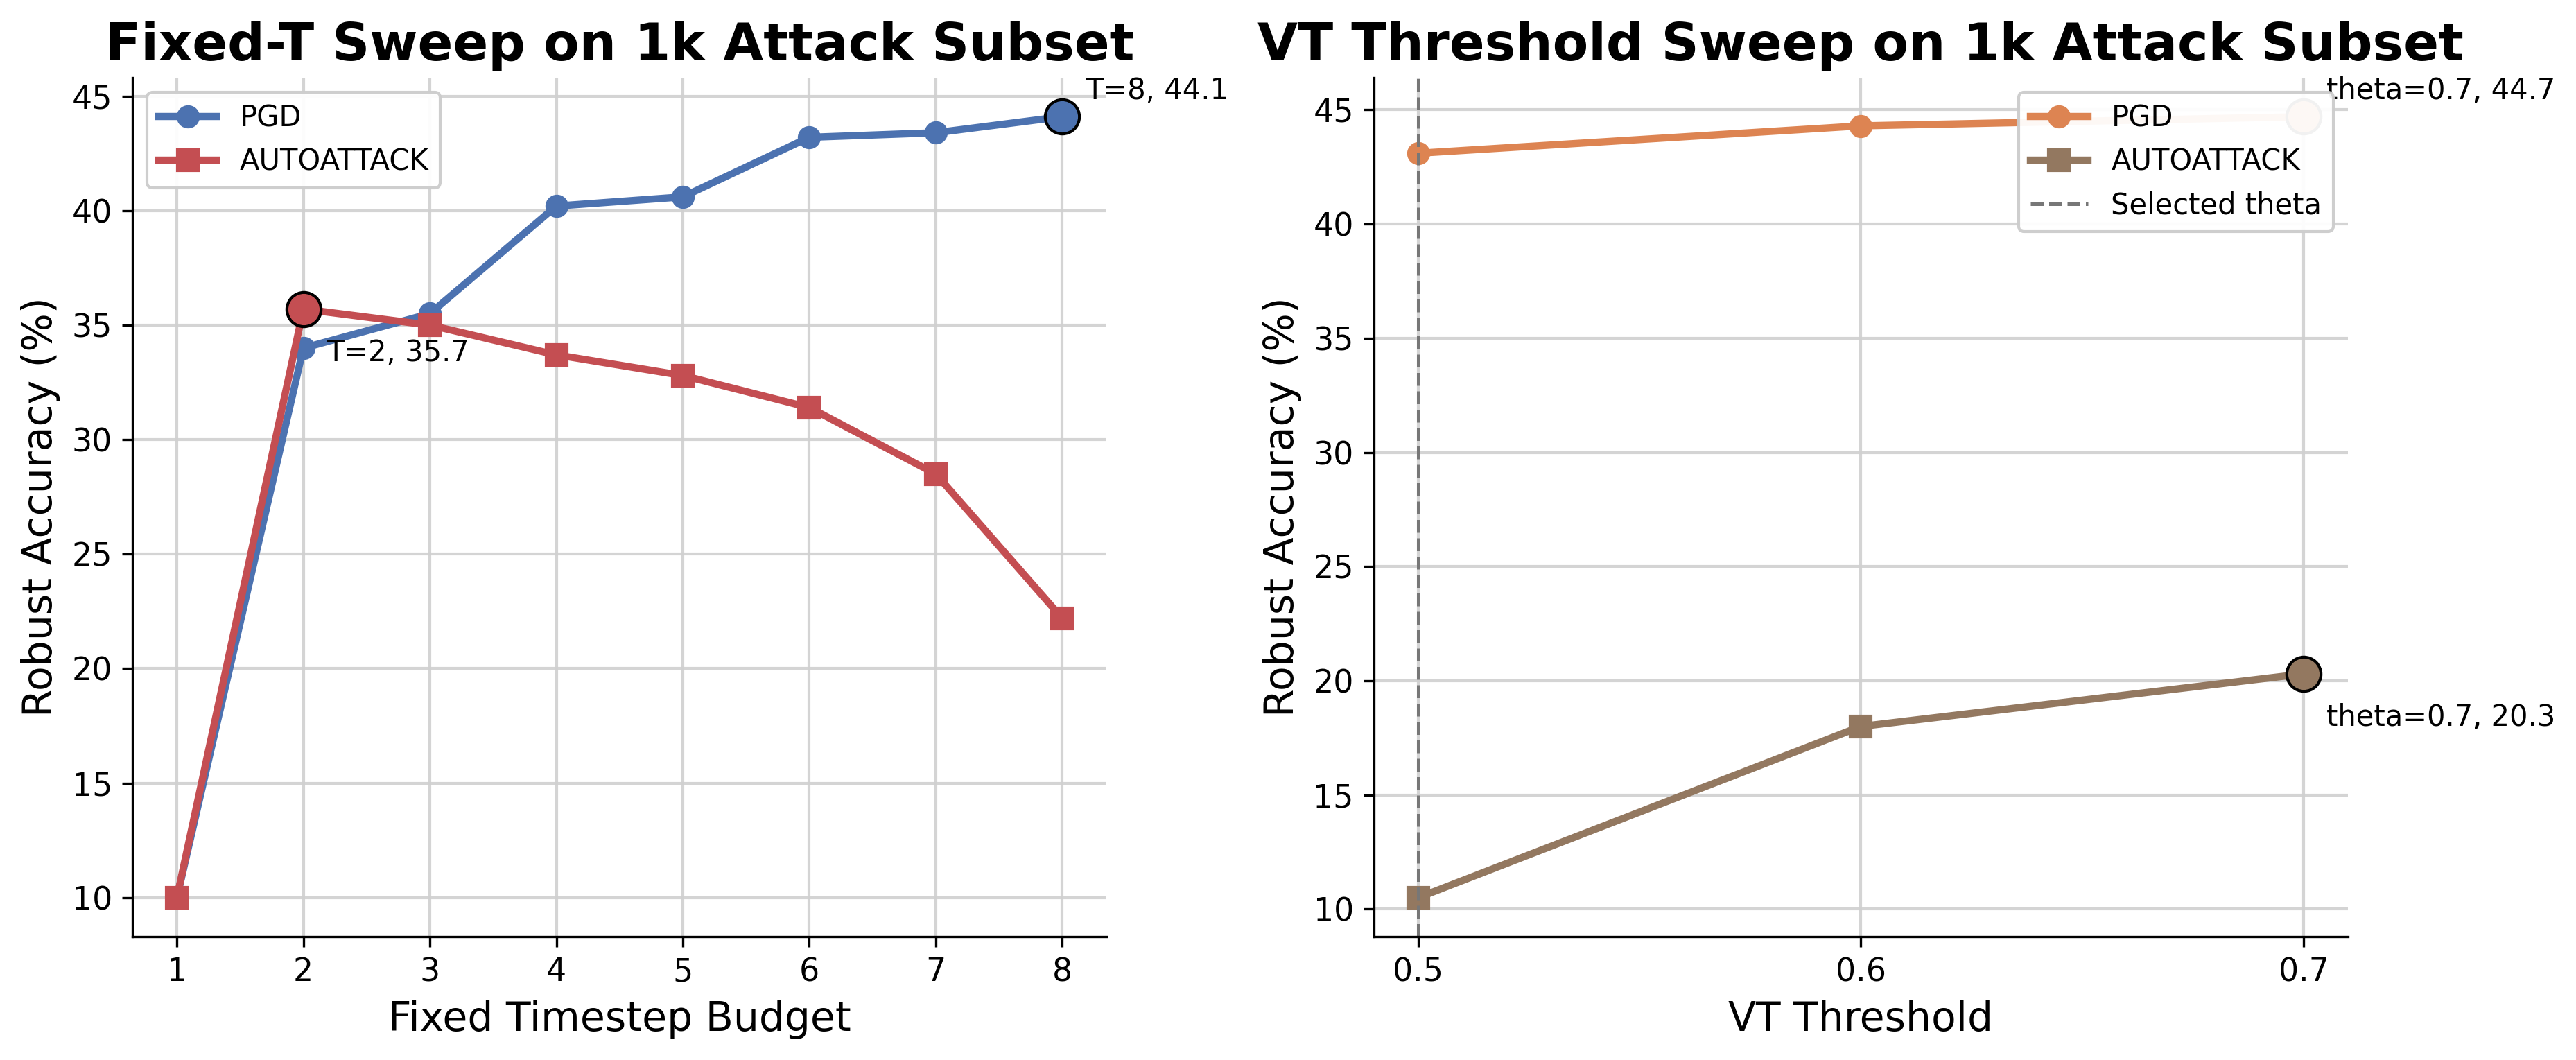
\includegraphics[width=0.96\linewidth]{paper_figures/fig_attack_sweep_subset.png}
\caption{Standalone adversarial-trained ResNet subset attack sweep. The left panel shows the full fixed-$T$ robustness sweep, directly addressing the concern that a different fixed horizon might be the true robust baseline. The right panel shows the corresponding VT threshold sweep on the same \num{1000}-sample subset.}
\label{fig:attack-sweep-standalone}
\end{figure}

\begin{table}[t]
\centering
\caption{Subset-based compute-matched robustness check for the adversarially trained models. On ResNet, the selected VT threshold $\theta=0.50$ is matched to fixed $T=4$ by clean SynOps. On VGG, the selected threshold $\theta=0.60$ is matched to fixed $T=6$. Results are from class-balanced \num{1000}-sample subsets.}
\label{tab:matched_control_robustness}
\begin{tabular}{llccc}
\toprule
Backbone & Attack & Fixed $T=8$ (\%) & Matched Fixed $T$ (\%) & VT Selected (\%) \\
\midrule
\multirow{2}{*}{ResNet-18} & PGD-20 untargeted & 44.1 & 40.2 ($T=4$) & 43.1 \\
 & AutoAttack & 22.2 & 33.7 ($T=4$) & 10.5 \\
\multirow{2}{*}{VGG16} & PGD-20 untargeted & 45.2 & 41.7 ($T=6$) & 45.9 \\
 & AutoAttack & 9.7 & 20.2 ($T=6$) & 8.2 \\
\bottomrule
\end{tabular}
\end{table}

\begin{table}[t]
\centering
\caption{Subset-based robustness sweep summary for the adversarially trained model. The fixed-$T$ and VT sweeps are evaluated on the same class-balanced \num{1000}-sample subset.}
\label{tab:subset_attack_sweep}
\begin{tabular}{lccc}
\toprule
Attack & Best Fixed-$T$ (\%) & Best VT Threshold (\%) & Selected VT (\%) \\
\midrule
PGD-20 untargeted & $T=8$: 44.1 & $\theta=0.70$: 44.7 & $\theta=0.50$: 43.1 \\
AutoAttack & $T=2$: 35.7 & $\theta=0.70$: 20.3 & $\theta=0.50$: 10.5 \\
\bottomrule
\end{tabular}
\end{table}

\subsection{Compute-Overuse Objectives Exploit Dynamic Halting}
Finally, we ask whether VT introduces a distinct compute-targeted vulnerability. The answer is yes.

The compute-overuse attack is not mainly a misclassification attack. Instead, it asks whether an adversary can force VT to spend more computation. On the ResNet case study, the clean-trained selected VT policy moves from a clean average stopping depth of 2.393 to 3.579 under compute-overuse attack. The adversarially trained selected policy moves from 4.332 to 4.698.

This implies that robustness for adaptive SNN inference should be treated as at least two partially separate questions:
\begin{itemize}[leftmargin=1.3em]
\item \textbf{label robustness:} does the prediction remain correct?
\item \textbf{compute robustness:} does the inference cost remain controlled?
\end{itemize}
However, this does not mean compute-overuse is the dominant failure mode in every regime; rather, it shows that VT can be attacked in more than one way and that robustness evaluation should not be reduced to label error alone. Figure~\ref{fig:regime-compute-overuse} shows the ResNet case study directly: the clean-trained model suffers a larger depth increase, while the adversarially trained model remains more label-stable under this objective.

\begin{figure}[t]
\centering
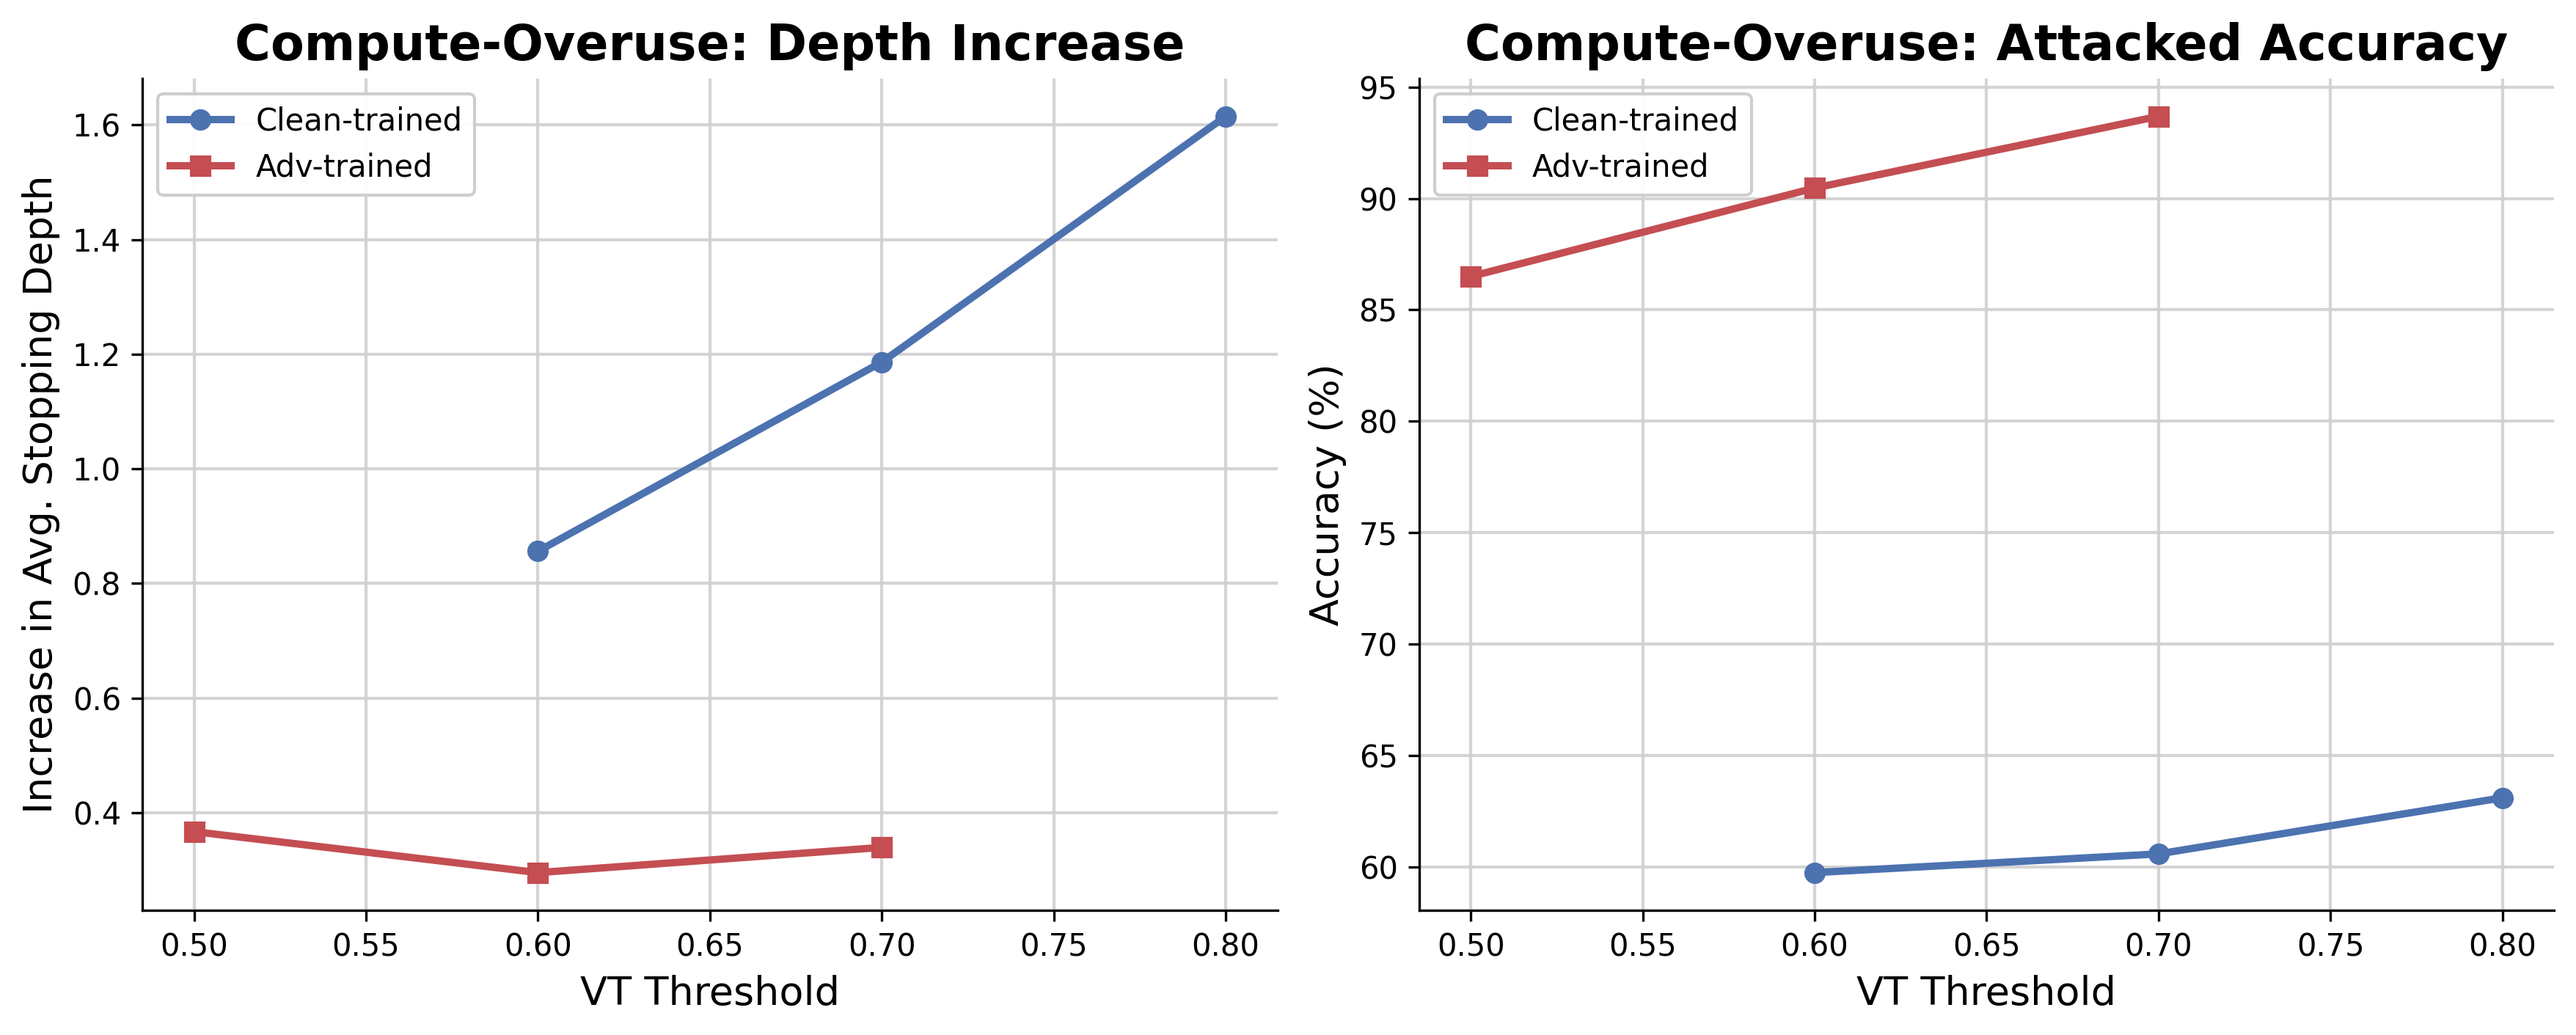
\includegraphics[width=\linewidth]{paper_figures/fig6_regime_compute_overuse.png}
\caption{Compute-overuse comparison across training regimes for the detailed ResNet case study. The clean-trained model experiences larger stopping-depth inflation, while the adversarially trained model retains higher attacked accuracy under the same objective.}
\label{fig:regime-compute-overuse}
\end{figure}

\section{Discussion}
\paragraph{What VT clearly does well.}
VT is an effective clean adaptive-inference mechanism. On both ResNet and VGG, and in both training regimes, it outperforms compute-matched fixed-time truncation on clean accuracy. This remains true even after adversarial training, although the size of the gain is reduced.

\paragraph{What VT does not automatically give.}
VT is not a universal robustness improvement. On the clean-trained models, there is essentially no robustness to preserve. On the adversarially trained models, VT can look favorable under PGD, especially relative to its compute-matched fixed-time control, but it is unfavorable under AutoAttack and does not beat the strongest fixed-time baselines. Any paper that claims a blanket robustness benefit from these results would be overstating the evidence.

\paragraph{Why the mixed result still matters.}
The value of the paper is precisely that it avoids collapsing these findings into a single slogan. VT is strong where it is supposed to be strong, namely on the clean efficiency frontier. The fact that PGD and AutoAttack do not agree is not an inconvenience to hide; it is evidence that adaptive inference should be evaluated more carefully than it often is.

\paragraph{What should change in how VT is evaluated.}
These experiments suggest that future VT studies should report compute-matched fixed-time controls by default, separate clean-trained from adversarially trained behavior, and avoid drawing robustness conclusions from one attack alone. When robustness is a core claim, fixed-$T$ sweeps should also be reported, because the strongest robust fixed-time operating point may differ substantially from both the clean-compute-matched control and the full-horizon baseline. That recommendation is supported directly by the present results rather than by conjecture.

\section{Limitations}
This draft has several limitations that should be stated directly.
\begin{itemize}[leftmargin=1.3em]
\item The paper now covers two deterministic backbones, vanilla ResNet-18 and vanilla VGG16, under both regimes. However, the deepest robustness sweep and most complete reviewer-facing attack study are still available only for ResNet. This limits how strongly we can generalize the fixed-$T$ sweep conclusions across architectures.
\item The paper evaluates one VT policy family rather than a broad space of adaptive stopping mechanisms. This limits claim scope, but it is consistent with the paper's goal, which is evaluation rather than method design.
\item For adversarially trained ResNet, the calibration-selected threshold sits at the lower edge of the current threshold grid. This may affect where the selected operating point lands, but it does not remove the broader frontier trend showing that VT still beats matched fixed-time controls.
\item Attack-side comparisons to matched fixed-time controls are currently strongest on class-balanced \num{1000}-sample subsets rather than the full \num{10000}-sample test set. This does not threaten the clean efficiency claim, but it does mean the strongest robustness fairness check should be interpreted as high-quality supporting evidence rather than as the final full-test result. The full fixed-$T$ sweep subset check is currently complete for ResNet but not for adversarially trained VGG because the last sweep timed out.
\end{itemize}

\section{Conclusion}
This paper asked a simple question: when VT is compared fairly against fixed-time truncation at similar clean compute budgets, what does it actually add, and does any such advantage extend from clean efficiency to adversarial robustness? The answer is that VT clearly improves the clean accuracy--compute frontier on both deterministic ResNet-18 and deterministic VGG16 SNNs, in both clean-trained and adversarially trained regimes, but its robustness behavior is conditional rather than automatic.

For the clean-trained models, VT is a strong efficiency mechanism but offers no meaningful robustness story. For the adversarially trained models, VT still improves the clean frontier and can even look favorable under PGD, but strong-attack evaluation shows that fixed-time baselines remain more robust than VT. The right takeaway is therefore neither triumphalist nor negative: VT is empirically valuable, but its added value is clearest beyond static truncation on the clean frontier, not as a general robustness improvement.

\begin{thebibliography}{99}

\bibitem{graves2016adaptive}
Alex Graves.
\newblock Adaptive computation time for recurrent neural networks.
\newblock \emph{arXiv preprint arXiv:1603.08983}, 2016.

\bibitem{teerapittayanon2016branchynet}
Surat Teerapittayanon, Bradley McDanel, and H.~T. Kung.
\newblock BranchyNet: Fast inference via early exiting from deep neural networks.
\newblock In \emph{International Conference on Pattern Recognition (ICPR)}, 2016.

\bibitem{huang2018msdnet}
Gao Huang, Danlu Chen, Tianhong Li, Felix Wu, Laurens van der Maaten, and Kilian Q. Weinberger.
\newblock Multi-scale dense networks for resource efficient image classification.
\newblock In \emph{International Conference on Learning Representations (ICLR)}, 2018.

\bibitem{li2023dynamicconfidence}
Yuhang Li et al.
\newblock Unleashing the potential of spiking neural networks by dynamic confidence.
\newblock In \emph{IEEE/CVF International Conference on Computer Vision (ICCV)}, 2023.

\bibitem{li2023dtsnn}
Yuhang Li et al.
\newblock Input-aware dynamic timestep spiking neural networks for efficient in-memory computing.
\newblock In \emph{Design Automation Conference (DAC)}, 2023.

\bibitem{chen2024spikecp}
Chen et al.
\newblock Knowing when to stop: Delay-adaptive spiking neural network classifiers with reliability guarantees.
\newblock \emph{arXiv preprint}, 2023.

\bibitem{rao2025vtsnn}
Rao et al.
\newblock VT-SNN: Variable time-step spiking neural network.
\newblock In \emph{International Conference on Medical Image Computing and Computer-Assisted Intervention (MICCAI)}, 2025.

\bibitem{rueckauer2017conversion}
Bodo Rueckauer, Iulia-Alexandra Lungu, Yuhuang Hu, Michael Pfeiffer, and Shih-Chii Liu.
\newblock Conversion of continuous-valued deep networks to efficient event-driven networks for image classification.
\newblock \emph{Frontiers in Neuroscience}, 11:682, 2017.

\bibitem{sorbaro2020energy}
Martino Sorbaro, Qian Liu, Massimo Bortone, and Sadique Sheik.
\newblock Optimizing the energy consumption of spiking neural networks for neuromorphic applications.
\newblock \emph{Frontiers in Neuroscience}, 14:662, 2020.

\bibitem{fang2021sewresnet}
Wei Fang, Zhaofei Yu, Yanqi Chen, Timothée Masquelier, Tiejun Huang, and Yonghong Tian.
\newblock Deep residual learning in spiking neural networks.
\newblock In \emph{Advances in Neural Information Processing Systems (NeurIPS)}, 2021.

\bibitem{deng2022tet}
Shikuang Deng, Yuhang Li, Shanghang Zhang, and Shi Gu.
\newblock Temporal efficient training of spiking neural network via gradient re-weighting.
\newblock In \emph{International Conference on Learning Representations (ICLR)}, 2022.

\bibitem{na2022autosnn}
Byunggook Na, Jisoo Mok, Seongsik Park, Donghyeon Lee, Hyeokjun Choe, and Sungroh Yoon.
\newblock AutoSNN: Towards energy-efficient spiking neural networks.
\newblock In \emph{International Conference on Machine Learning (ICML)}, 2022.

\bibitem{sharmin2019comprehensive}
Saima Sharmin et al.
\newblock A comprehensive analysis on adversarial robustness of spiking neural networks.
\newblock In \emph{International Joint Conference on Neural Networks (IJCNN)}, 2019.

\bibitem{sharmin2020inherent}
Saima Sharmin et al.
\newblock Inherent adversarial robustness of deep spiking neural networks: Effects of discrete input encoding and non-linear activations.
\newblock In \emph{European Conference on Computer Vision (ECCV)}, 2020.

\bibitem{liang2022toward}
Ling Liang et al.
\newblock Toward robust spiking neural network against adversarial perturbation.
\newblock \emph{arXiv preprint arXiv:2205.01625}, 2022.

\bibitem{wu2024rscsnn}
Wu et al.
\newblock RSC-SNN: Exploring the trade-off between adversarial robustness and accuracy in spiking neural networks via randomized smoothing coding.
\newblock \emph{arXiv preprint arXiv:2407.20099}, 2024.

\bibitem{wang2025randhet}
Jihang Wang et al.
\newblock Random heterogeneous spiking neural network for adversarial defense.
\newblock \emph{iScience}, 2025.

\bibitem{ding2025neuromorphic}
Ding et al.
\newblock Neuromorphic computing paradigms enhance robustness through spiking neural networks.
\newblock \emph{Nature Communications}, 2025.

\bibitem{madry2018pgd}
Aleksander Madry, Aleksandar Makelov, Ludwig Schmidt, Dimitris Tsipras, and Adrian Vladu.
\newblock Towards deep learning models resistant to adversarial attacks.
\newblock In \emph{International Conference on Learning Representations (ICLR)}, 2018.

\bibitem{athalye2018obfuscated}
Anish Athalye, Nicholas Carlini, and David Wagner.
\newblock Obfuscated gradients give a false sense of security: Circumventing defenses to adversarial examples.
\newblock In \emph{International Conference on Machine Learning (ICML)}, 2018.

\bibitem{croce2020autoattack}
Francesco Croce and Matthias Hein.
\newblock Reliable evaluation of adversarial robustness with an ensemble of diverse parameter-free attacks.
\newblock In \emph{International Conference on Machine Learning (ICML)}, 2020.

\bibitem{tramer2020adaptive}
Florian Tramèr, Nicholas Carlini, Wieland Brendel, and Aleksander Madry.
\newblock On adaptive attacks to adversarial example defenses.
\newblock In \emph{Advances in Neural Information Processing Systems (NeurIPS)}, 2020.

\bibitem{wang2025reliableeval}
Wang et al.
\newblock Towards reliable evaluation of adversarial robustness for spiking neural networks.
\newblock \emph{arXiv preprint}, 2025.

\end{thebibliography}

\end{document}
